
%       Process with LaTeX  (Tested on LaTeX 2e pdflatex)

\documentclass{article}
\newfont{\atlsub}{cmssi17}
\newfont{\cmt}{cmssi8}

\usepackage{aitech}
\usepackage{atldoc}
\usepackage{alltt}
\usepackage{graphicx}

\begin{document}

\title{ClassWar \\
\vspace{10pt}
{\LARGE \sf Class Language Application Support System Within AutoCAD\@.
Really!} \\
\vspace{10pt}
$\overline{\makebox{\underline{\atlsub An Atlast Application}}}$
}

\abstract{
    An embedded object oriented programming environment implements
    user-defined entities in AutoCAD\@.  Both
    objects and methods are completely portable.
    Optionally, methods can be implemented in C to protect proprietary
    algorithms or maximise performance.
}
\author{John Walker}
\date{May 6th, 1990}

\maketitle

% psfigTeX macros
%
% All software, documentation, and related files in this distribution of
% psfig/tex are Copyright (c) 1987 Trevor J. Darrell
%
% Permission is granted for use and non-profit distribution of psfig/tex
% providing that this notice be clearly maintained, but the right to
% distribute any portion of psfig/tex for profit or as part of any commercial
% product is specifically reserved for the author.
%
%
% $Header: psfig.tex,v 1.7 87/01/19 15:55:27 trevor Exp $
%
\catcode`\@=11\relax
\newwrite\@unused
\def\typeout#1{{\let\protect\string\immediate\write\@unused{#1}}}
\def\psglobal#1{
\immediate\special{ps:plotfile #1 global}}
\def\psfiginit{\typeout{psfiginit}
\immediate\psglobal{figtex.pro}}
%
% @psdo control structure -- similar to Latex @for.
% I redefined these with different names so that psfig can
% be used with TeX as well as LaTeX, and so that it will not
% be vunerable to future changes in LaTeX's internal
% control structure,
%
\def\@nnil{\@nil}
\def\@empty{}
\def\@psdonoop#1\@@#2#3{}
\def\@psdo#1:=#2\do#3{\edef\@psdotmp{#2}\ifx\@psdotmp\@empty \else
    \expandafter\@psdoloop#2,\@nil,\@nil\@@#1{#3}\fi}
\def\@psdoloop#1,#2,#3\@@#4#5{\def#4{#1}\ifx #4\@nnil \else
       #5\def#4{#2}\ifx #4\@nnil \else#5\@ipsdoloop #3\@@#4{#5}\fi\fi}
\def\@ipsdoloop#1,#2\@@#3#4{\def#3{#1}\ifx #3\@nnil
       \let\@nextwhile=\@psdonoop \else
      #4\relax\let\@nextwhile=\@ipsdoloop\fi\@nextwhile#2\@@#3{#4}}
\def\@tpsdo#1:=#2\do#3{\xdef\@psdotmp{#2}\ifx\@psdotmp\@empty \else
    \@tpsdoloop#2\@nil\@nil\@@#1{#3}\fi}
\def\@tpsdoloop#1#2\@@#3#4{\def#3{#1}\ifx #3\@nnil
       \let\@nextwhile=\@psdonoop \else
      #4\relax\let\@nextwhile=\@tpsdoloop\fi\@nextwhile#2\@@#3{#4}}
%
%
\def\psdraft{
       \def\@psdraft{0}
       %\typeout{draft level now is \@psdraft \space . }
}
\def\psfull{
       \def\@psdraft{100}
       %\typeout{draft level now is \@psdraft \space . }
}
\psfull
\newif\if@prologfile
\newif\if@postlogfile
%%% These are for the option list.
%%% A specification of the form a = b maps to calling \@p@@sa{b}
\newif\if@bbllx
\newif\if@bblly
\newif\if@bburx
\newif\if@bbury
\newif\if@height
\newif\if@width
\newif\if@rheight
\newif\if@rwidth
\newif\if@clip
\def\@p@@sclip#1{\@cliptrue}
\def\@p@@sfile#1{%\typeout{file is #1}
                  \def\@p@sfile{#1}
}
\def\@p@@sfigure#1{\def\@p@sfile{#1}}
\def\@p@@sbbllx#1{
               %\typeout{bbllx is #1}
               \@bbllxtrue
               \dimen100=#1
               \edef\@p@sbbllx{\number\dimen100}
}
\def\@p@@sbblly#1{
               %\typeout{bblly is #1}
               \@bbllytrue
               \dimen100=#1
               \edef\@p@sbblly{\number\dimen100}
}
\def\@p@@sbburx#1{
               %\typeout{bburx is #1}
               \@bburxtrue
               \dimen100=#1
               \edef\@p@sbburx{\number\dimen100}
}
\def\@p@@sbbury#1{
               %\typeout{bbury is #1}
               \@bburytrue
               \dimen100=#1
               \edef\@p@sbbury{\number\dimen100}
}
\def\@p@@sheight#1{
               \@heighttrue
               \dimen100=#1
               \edef\@p@sheight{\number\dimen100}
               %\typeout{Height is \@p@sheight}
}
\def\@p@@swidth#1{
               %\typeout{Width is #1}
               \@widthtrue
               \dimen100=#1
               \edef\@p@swidth{\number\dimen100}
}
\def\@p@@srheight#1{
               %\typeout{Reserved height is #1}
               \@rheighttrue
               \dimen100=#1
               \edef\@p@srheight{\number\dimen100}
}
\def\@p@@srwidth#1{
               %\typeout{Reserved width is #1}
               \@rwidthtrue
               \dimen100=#1
               \edef\@p@srwidth{\number\dimen100}
}
\def\@p@@sprolog#1{\@prologfiletrue\def\@prologfileval{#1}}
\def\@p@@spostlog#1{\@postlogfiletrue\def\@postlogfileval{#1}}
\def\@cs@name#1{\csname #1\endcsname}
\def\@setparms#1=#2,{\@cs@name{@p@@s#1}{#2}}
%
% initialize the defaults (size the size of the figure)
%
\def\ps@init@parms{
               \@bbllxfalse \@bbllyfalse
               \@bburxfalse \@bburyfalse
               \@heightfalse \@widthfalse
               \@rheightfalse \@rwidthfalse
               \def\@p@sbbllx{}\def\@p@sbblly{}
               \def\@p@sbburx{}\def\@p@sbbury{}
               \def\@p@sheight{}\def\@p@swidth{}
               \def\@p@srheight{}\def\@p@srwidth{}
               \def\@p@sfile{}
               \def\@p@scost{10}
               \def\@sc{}
               \@prologfilefalse
               \@postlogfilefalse
               \@clipfalse
}
%
% Go through the options setting things up.
%
\def\parse@ps@parms#1{
               \@psdo\@psfiga:=#1\do
                  {\expandafter\@setparms\@psfiga,}}
%
% Compute bb height and width
%
\newif\ifno@bb
\newif\ifnot@eof
\newread\ps@stream
\def\bb@missing{
       %\typeout{psfig: searching \@p@sfile \space  for bounding box}
       \openin\ps@stream=\@p@sfile
       \no@bbtrue
       \not@eoftrue
       \catcode`\%=12
       \loop
               \read\ps@stream to \line@in
               \global\toks200=\expandafter{\line@in}
               \ifeof\ps@stream \not@eoffalse \fi
               %\typeout{ looking at :: \the\toks200 }
               \@bbtest{\toks200}
               \if@bbmatch\not@eoffalse\expandafter\bb@cull\the\toks200\fi
       \ifnot@eof \repeat
       \catcode`\%=14
}
\catcode`\%=12
\newif\if@bbmatch
\def\@bbtest#1{\expandafter\@a@\the#1%%BoundingBox:\@bbtest\@a@}
\long\def\@a@#1%%BoundingBox:#2#3\@a@{\ifx\@bbtest#2\@bbmatchfalse\else\@bbmatchtrue\fi}
\long\def\bb@cull#1 #2 #3 #4 #5 {
       \dimen100=#2 bp\edef\@p@sbbllx{\number\dimen100}
       \dimen100=#3 bp\edef\@p@sbblly{\number\dimen100}
       \dimen100=#4 bp\edef\@p@sbburx{\number\dimen100}
       \dimen100=#5 bp\edef\@p@sbbury{\number\dimen100}
       \no@bbfalse
}
\catcode`\%=14
%
\def\compute@bb{
               \no@bbfalse
               \if@bbllx \else \no@bbtrue \fi
               \if@bblly \else \no@bbtrue \fi
               \if@bburx \else \no@bbtrue \fi
               \if@bbury \else \no@bbtrue \fi
               \ifno@bb \bb@missing \fi
               \ifno@bb \typeout{FATAL ERROR: no bb supplied or found}
                       \no-bb-error
               \fi
               %
               \count203=\@p@sbburx
               \count204=\@p@sbbury
               \advance\count203 by -\@p@sbbllx
               \advance\count204 by -\@p@sbblly
               \edef\@bbw{\number\count203}
               \edef\@bbh{\number\count204}
               %\typeout{ bbh = \@bbh, bbw = \@bbw }
}
%
% \in@hundreds performs #1 * (#2 / #3) correct to the hundreds,
%      then leaves the result in @result
%
\def\in@hundreds#1#2#3{\count240=#2 \count241=#3
                    \count100=\count240        % 100 is first digit #2/#3
                    \divide\count100 by \count241
                    \count101=\count100
                    \multiply\count101 by \count241
                    \advance\count240 by -\count101
                    \multiply\count240 by 10
                    \count101=\count240        %101 is second digit of #2/#3
                    \divide\count101 by \count241
                    \count102=\count101
                    \multiply\count102 by \count241
                    \advance\count240 by -\count102
                    \multiply\count240 by 10
                    \count102=\count240        % 102 is the third digit
                    \divide\count102 by \count241
                    \count200=#1\count205=0
                    \count201=\count200
                       \multiply\count201 by \count100
                       \advance\count205 by \count201
                    \count201=\count200
                       \divide\count201 by 10
                       \multiply\count201 by \count101
                       \advance\count205 by \count201
                       %
                    \count201=\count200
                       \divide\count201 by 100
                       \multiply\count201 by \count102
                       \advance\count205 by \count201
                       %
                    \edef\@result{\number\count205}
}
\def\compute@wfromh{
               % computing : width = height * (bbw / bbh)
               \in@hundreds{\@p@sheight}{\@bbw}{\@bbh}
               %\typeout{ \@p@sheight * \@bbw / \@bbh, = \@result }
               \edef\@p@swidth{\@result}
               %\typeout{w from h: width is \@p@swidth}
}
\def\compute@hfromw{
               % computing : height = width * (bbh / bbw)
               \in@hundreds{\@p@swidth}{\@bbh}{\@bbw}
               %\typeout{ \@p@swidth * \@bbh / \@bbw = \@result }
               \edef\@p@sheight{\@result}
               %\typeout{h from w : height is \@p@sheight}
}
\def\compute@handw{
               \if@height
                       \if@width
                       \else
                               \compute@wfromh
                       \fi
               \else
                       \if@width
                               \compute@hfromw
                       \else
                               \edef\@p@sheight{\@bbh}
                               \edef\@p@swidth{\@bbw}
                       \fi
               \fi
}
\def\compute@resv{
               \if@rheight \else \edef\@p@srheight{\@p@sheight} \fi
               \if@rwidth \else \edef\@p@srwidth{\@p@swidth} \fi
}
%
% Compute any missing values
\def\compute@sizes{
       \compute@bb
       \compute@handw
       \compute@resv
}
%
% \psfig
% usage : \psfig{file=, height=, width=, bbllx=, bblly=, bburx=, bbury=,
%                      rheight=, rwidth=, clip=}
%
% "clip=" is a switch and takes no value, but the `=' must be preset.
\def\psfig#1{\vbox {
       % do a zero width hard space so that a single
       % \psfig in a centering enviornment will behave nicely
       %{\setbox0=\hbox{\ }\ \hskip-\wd0}
       %
       \ps@init@parms
       \parse@ps@parms{#1}
       \compute@sizes
       %
       \ifnum\@p@scost<\@psdraft{
               %\typeout{psfig: including \@p@sfile \space }
               %
               \special{ps::[begin]    \@p@swidth \space \@p@sheight \space
                               \@p@sbbllx \space \@p@sbblly \space
                               \@p@sbburx \space \@p@sbbury \space
                               startTexFig \space }
               \if@clip{
                       \typeout{(clip)}
                       \special{ps:: \@p@sbbllx \space \@p@sbblly \space
                               \@p@sbburx \space \@p@sbbury \space
                               doclip \space }
               }\fi
               \if@prologfile
                   \special{ps: plotfile \@prologfileval \space } \fi
               \special{ps: plotfile \@p@sfile \space }
               \if@postlogfile
                   \special{ps: plotfile \@postlogfileval \space } \fi
               \special{ps::[end] endTexFig \space }
               % Create the vbox to reserve the space for the figure
               \vbox to \@p@srheight true sp{
                       \hbox to \@p@srwidth true sp{
                               \hfil
                       }
               \vfil
               }
       }\else{
               % draft figure, just reserve the space and print the
               % path name.
               \vbox to \@p@srheight true sp{
               \vss
                       \hbox to \@p@srwidth true sp{
                               \hss
                               \@p@sfile
                               \hss
                       }
               \vss
               }
       }\fi
}}
\catcode`\@=12\relax


\newcommand{\atlas}{\underline{\underline{\sc Atlast}}}
\newcommand{\cw}{{\sc ClassWar}}
\hyphenation{Auto-CAD Auto-Lisp Auto-Shade}

\begin{quote}
    The world is divided into two classes, those who believe the
    incredible, and those who do the improbable.

\vspace{-1ex}
\raggedleft
{\sc Oscar Wilde, 1893}
\end{quote}

\dcap{S}TARTING {\sc with the original} prototype of AutoLisp in
1984, we've been moving toward providing general user-defined entities
in AutoCAD\@.  Even though the goal was clear, we knew that much
groundwork would be necessary before AutoCAD could provide its users
such a facility.  We needed a high performance programming language,
since AutoLisp was far too slow for applications more computationally
intense than macro language usage, and we needed a memory architecture
that would provide the storage required by a compiled language.  We
needed to extend our original ASCII attributes for blocks to allow
efficient binary storage of arbitrary attributes on any entity.  We
needed to permit applications to create AutoCAD objects far more
efficiently than by submitting commands.  And finally, we
needed a way to embed object definitions within an AutoCAD database so
user-defined entities would be just as transportable as block
definitions.

During the development of Release 11, essentially all of the long-term
goals we've been working toward for so long have been accomplished.  The
development of AutoCAD 386 and AutoCAD for OS/2 have made large memory
architectures readily accessible to the overwhelming majority of our
customer base, freeing us of the extensibility and performance
shackles of the original MS-DOS memory architecture (all other AutoCAD
implementations are, and have been since inception, large memory
architectures).  With adequate storage at hand, ADS provided
access to AutoCAD facilities from compiled C code, eliminating the
interpretive overhead of AutoLisp.  Extended Entity Data (entity
attributes) allowed applications to attach a wide variety of
application data to database objects, data automatically
adjusted by AutoCAD when the object undergoes affine transformations.
The \verb+ads_entmake()+ facility, along with its ability to
dynamically create anonymous geometry blocks, provides a high
performance way for applications to add objects to an AutoCAD
database.

The realisation that these features enabled applications to extend the
basic entity repertoire of AutoCAD in a coherent, almost seamless way, led to
the original Eagle integrated solid modeling prototype project, which
has resulted in the development of the AME solid modeling
package now scheduled for shipment with AutoCAD Release 11.
Several subsequent projects to add more powerful modeling and analysis
capabilities to AutoCAD, such as NURBS, a constraint manager, and 2D
CSG and FEM, also exploit these facilities to extend AutoCAD\@.

These projects have demonstrated that AutoCAD is extensible through
the addition of C coded applications that embody the calculation code
for their speciality, but store their data in an AutoCAD database and
rely on AutoCAD for user interface and for common geometrical
operations.  While this has gone a long way toward our original goals
for user-defined objects, some desiderata remain undone.  To extend
AutoCAD's philosophy of open architecture fully into the domain of
application-defined objects, we need to adopt many of the principles
which have become the goals of ``object oriented programming,''
embodying them in the structure we encourage (but do not require)
application developers to use.  By providing this framework we can
promote interoperability among applications, allow users to build upon
applications just as they have done with the primitives provided by
AutoCAD, eliminate the penalty for objects defined outside the
``AutoCAD core,'' and hence avert the need for it to grow in size and
complexity through time. We can allow developers to draw the line between
the open and proprietary parts of their applications at
will---governed by their strategy and the norms of the marketplace
rather than by a rigid set of rules laid down by our implementation.

\cw\ ({\sf Class Language Application Support System Within
AutoCAD, Really!})\ is an attempt to achieve all of these goals, to
fuse the methodologies of object oriented programming with those of
geometric modeling, to create an application environment of reusable
pieces where users and developers can easily create customised
modeling environments by selecting and combining components, and to
avert the chaotic and bewildering consequences that seem
inevitable were hundreds of mutually incompatible applications to
emerge.  Building upon the new AutoCAD facilities in Release 11 and
incorporating many of the software components I've been developing for
the last several years against this day, \cw\ provides
a true object oriented framework for AutoCAD applications, one that
will automatically and compatibly benefit from the internal
restructuring of AutoCAD along object oriented lines anticipated in
the next several major releases.

In the large, \cw\ can be seen as a unifying framework for all
AutoCAD applications, bestowing the benefits of interoperability and
user extensibility upon all that conform to its standards.  In the
small, \cw\ is an ADS application which can be shipped in
either binary or source code form with AutoCAD Release 11 which allows
simple user-defined entities to be created, manipulated, and exchanged
among users.  These views describe the same piece of software; the
distinction is one of perception, strategy, and consequent market
positioning.  I am confident enough in the wisdom of our users that
I'm sure that regardless of how much or how little fanfare accompanies the
delivery of \cw\ into their hands, they will rapidly determine its
true value and apply it accordingly.

\section{\cw\ Overview}

{\bf Note:} {\sl To those experienced with conventional AutoCAD
applications, or familiar with object oriented programming languages
but not AutoCAD, the concepts of \cw\ may seem alien and difficult to
master.  \cw\ is a system in which much of the power is implicit in
its programmability and the ability to build on previously-defined
components.  Like most such systems it may be difficult to come up
to speed in its use from a description of its commands and language
features.  To assist in mastering the system, I produced a 90 minute
video demonstration titled ``{\cw---{\sc The Video}}.''  An NTSC/VHS copy
of this tape is available in the Autodesk technical library in
Sausalito.  Notwithstanding the tacky production values and crashingly
boring dramatic merits of this opus, I highly recommend you view it
before reading this document.}

\subsection{Basic concepts}

\paragraph{Classes.}
\cw\ defines and manipulates user-defined entities which are
stored in the AutoCAD database.  Each of these entities is an {\em
instance} of a {\em class}.  The entity consists of an AutoCAD
anonymous block definition and a single insertion of it; the block
definition contains the (possibly void) geometrical object specified
by this instance.  Attached to the insertion of the block are extended
entity data which contain the {\em instance variables} specifying the
object.  The definition of these variables, the relationship between
them and the geometry of the object, and all operations which
manipulate
them are given in the {\em class definition}.  The class definition
is specified by a block in the same drawing that contains instances of
it.  The class definition can either contain the actual \cw\ source
code defining the class, or can reference a definition of the class
given in an ASCII text file.  A class definition consists of
declarations of its instance variables, which specify the properties of
a specific instance, its {\em class variables}, which store data
common to all instances of the class, and {\em method definitions}:
executable \cw\ code specifying the operations
that manipulate instances of the class.

\paragraph{Methods.}
Method definitions can either be given as source code within the class
definition or can be {\em external methods}, implemented in other ADS
applications and called with \verb+ads_invoke()+.  Methods, however
specified, can be invoked from within other \cw\ programs or, if
declared as {\em command methods}, can be called as an AutoCAD command
with the method's name.  Methods can have {\em arguments} which
are passed on the \atlas\ stack when they're invoked within programs
and obtained by prompting the user when the method is used as an
AutoCAD command.  Any number of different class definitions may
define methods with the same name; \cw\ automatically executes
the correct method based on the class an object belongs to.
Methods used as AutoCAD commands may be applied to selection
sets containing objects of different classes, and \cw\ will obtain the
information from the user required by the union of the argument lists
of the method definitions for all objects in the selection set,
combining identical argument requests to avoid duplication, and then
run the correct method for each selected object, passing it the
arguments it expects.

\paragraph{Variables.}
Class and instance variables may be either {\em primitive data types},
which include all the data types representable as AutoCAD entity
attributes (such as real numbers, integers, strings, distances,
locations in 3-space, orientation vectors, scale factors, etc.),\ or
instances of other classes.  The ability to include class instances
within other class definitions allows assembling composite objects
from previously defined pieces.  When an instance is included within
another class definition, all of its {\em public} methods may be
applied to it by methods of the class including it.

\paragraph{Inheritance.}
Class definitions may {\em inherit} (or, in other words, be {\em
derived from}), previously defined classes.  When a class inherits
the properties of another, it contains all the instance and class
variables, and methods of its {\em parent} class, although some of
these may not be directly accessible if declared {\em private} in the
parent class definition.  {\em Protected} methods and data are
accessible to classes derived from the parent, but not to those that
simply include instances of the class---they may use only {\em public}
items.  A derived class inherits all the methods of the parent class,
but may redefine, or {\em overload}, any of them with a method of its
own, should the derived class wish a different action for that method.
Even if a method is overloaded, the parent's method with the same name
may still be called by explicitly specifying invocation of that method.
A derived class may either allow all the methods of the parent to
``show through,'' in which case the class is considered {\em
publicly} derived, or may {\em encapsulate} (hide) them, being then
deemed {\em privately} derived.

\paragraph{Constructors.}
A class definition may specify a {\em class constructor} or {\em
newclass method}, executed when the class is initially
defined; this method is frequently used to initialise class variables.
In addition, an {\em instance constructor}, or {\em new method}, can be
specified.  It is executed whenever a new instance of the class is
created and typically sets instance variables to default values for
new objects of that class.  If a class definition contains an {\em
acquire method}, an AutoCAD user can create instances of the class
simply by entering the class name as an AutoCAD command.  The acquire
method normally prompts the user for information that defines the
instance.

\paragraph{Geometry.}
Most class instances will have a geometrical representation that is
visible and manipulable with AutoCAD (although this is not required).
A class definition specifies the geometry that represents it in its {\em
draw method}, automatically invoked when an instance of the
class is created or modified.  The draw method can create AutoCAD
geometry using three distinct facilities, or any combination thereof.
The most basic mechanism provides direct access to the
\verb+ads_entmake()+ facilities of ADS\@.  A set of \atlas\
definitions collectively referred to as the {\em \atlas\ ADS bindings}
allow method code to assemble result item chains and enter them in the
database.  The ADS bindings are derived from, and essentially
compatible with, the mechanisms introduced for manipulating DXF
information in {\tt DXFIX}\@.  The ADS binding package allows access
to all objects in AutoCAD's repertoire and precise control over the
entities created, but requires corresponding care on the user's part
to achieve the desired results.  A higher level of abstraction is
provided by the second geometric definition facility, the {\em SGLIB
binding}.  This package provides \atlas\ definitions for all the
functions of my C language Simple Graphics Library, providing both
comprehensive three dimensional linear algebra and geometric
facilities, plus tools for generating vectors, faces, meshes, and
commonly used objects including all the regular polyhedra and spheres.
The linear algebra components of the SGLIB package can be used to
calculate components for the lower level ADS package as well.
The highest level of geometry creation is embodied in the {\em turtle
geometry package}.  Based upon the turtle procedure notation given
in the book {\sl Turtle Geometry},\footnote{Harold Abelson \& Andrea
diSessa, {\em Turtle Geometry}, MIT Press: Cambridge (Mass), 1980,
1986.} but extended to three dimensions along the guidelines given in that
book, one or more turtles can be used to construct arbitrary geometric
features, ``leaving tracks'' as they draw either in the form of
ephemeral vectors that disappear on the next {\tt REDRAW}, Lines,
Polylines, or polygonal faces traced out by the turtle as closed
polygons.  The turtles provided by \cw\ are neither teenage, mutant,
nor Ninja.

\section{Using \cw}

Installing \cw\ in your AutoCAD environment and using it is relatively
simple; the power of \cw\ comes from the classes you create using it,
not from its built in commands.  To activate \cw , use
the AutoCAD command:

\verb+(xload "class")+

to load the application.  If you want \cw\ automatically loaded
whenever you run AutoCAD, add it to the list of standard applications
in your {\tt acad.ads} file.  After \cw\ is loaded, it immediately
reads configuration information and the definition of the ``object
superclass'' from the files {\tt config.cls} and {\tt object.cls}
respectively.  These files are supplied with \cw\ and should not be
modified as they interact intimately with the {\tt class} application
(substantial parts of \cw\ are written in its own programming language
and are contained in these files).  The {\tt config.cls} and {\tt
object.cls} files may be placed anywhere on AutoCAD's search path, and are
normally kept with other support files such as {\tt acad.pat} and {\tt
acad.lin}.

\cw\ stores class definitions in a temporary memory area called the
``heap.'' The heap must be sufficiently large to simultaneously hold
all the class definitions used by a drawing.  If the heap is too
small, \cw\ will run out of memory attempting to compile the class
definitions and will disable all class commands for the duration
of that drawing editor session.  The heap is specified in terms of
items, each 4 bytes in length.  The default heap size of 5000 items
(20K bytes) is adequate for most simple class definitions.  You
can specify the heap size by defining the environment variable ``{\tt
CLASSHEAP}'' as the desired heap size in items.  To determine how much
heap is used by the classes referenced by a drawing, enter the command
``{\tt /~MEMSTAT}'' at the AutoCAD command prompt after all classes
have been loaded.  Be sure to include the blank after the slash in
this command.  Class definitions are stored in a very compact form, so
large amounts of heap are rarely required except for classes that
contain large amounts of floating point co-ordinate data.

\subsection{Loading classes}

You can define classes interactively within the AutoCAD drawing editor
or import their definitions from text files prepared with your
favourite text editor.  Classes can be stored either within the
AutoCAD drawing file or externally in text files.

\subsubsection{The {\tt CLASSDEF} command}

The {\tt CLASSDEF} command defines a class whose definition is stored
within the AutoCAD drawing file.  If all class definitions used by
a drawing are embedded within it, and you send the {\tt .dwg}
file to another AutoCAD user who's installed \cw , that user can
perform all the operations defined by the embedded classes.

To define an embedded class, enter the {\tt CLASSDEF} command.
AutoCAD presents you with an attribute editing window.  Enter the
class name in the first line of this window; the class name must not
duplicate the name of any other class in the drawing, and should
conform to AutoCAD's conventions for object names (such as layer, line
type, and block names).

You can either directly type the class definition in to this window,
using the \cw\ programming language described later in
this document, or import a class definition in that language from an
external text file.  To load a text file, enter:

{\tt <}{\em filename}

as the first line of the class definition.  When you pick {\tt OK},
the class definition will be loaded from the named file.  If no
explicit path is specified in {\em filename}, it is searched for using
the same search path AutoCAD uses for block insertions.  If no
extension is given {\tt .cls} is used.  Files loaded with this
mechanism may use any of the end of line conventions accepted by
AutoCAD for text files it reads.

\subsubsection{The {\tt CLASSFILE} command}

Classes defined with {\tt CLASSDEF} are stored within the AutoCAD
drawing file.  While this makes the drawing self-contained and easy to
interchange with other users, it may prove inefficient if lengthy
class definitions are included in a large collection of drawings.  In
addition, in some environments users may want to maintain a standard
library of class definitions in a central repository
so updates to the master set of classes immediately
affect any drawing that uses one of them.

The {\tt CLASSFILE} command defines a class used within a drawing
but defined in an external text file.  Every time the drawing is
edited, the class definition is loaded from the text file.  If the
class definition file cannot be located when the drawing is edited
(for example, you've sent the drawing to another user but forgotten to
include one of the class definitions it uses), normal AutoCAD commands
will be able to manipulate objects of that class but all
object-specific commands defined in the class definition will be
unavailable.

To declare a class defined in a text file, enter the {\tt CLASSFILE}
command.  AutoCAD presents you with an attribute edit box requesting
the class name and the file where it is defined.  Enter the class
name, which must be a valid AutoCAD symbol name not used by any
previously-defined class, and the file name containing the class
definition.  If you leave the file name blank, the class will be
loaded from a file with the same name as the class with the default
extension of {\tt .cls} appended, located using the AutoCAD search
path.  If a file name is given, the AutoCAD search path is
used to find it unless an explicit path is specified.  Class
definition files may use any of the end of line conventions accepted
by AutoCAD\@.

\subsection{Editing classes: the {\tt CLASSEDIT} command}

The {\tt CLASSEDIT} command allows you to modify the definition of any
class embedded within a drawing (defined with {\tt CLASSDEF}), or
direct a class definition in an external text file to load a
different file.  Enter the {\tt CLASSEDIT} command, and AutoCAD will
prompt you:

{\tt Select class instance, or CR to name class:}

The easiest way to specify which class you wish to edit is just to
pick an object of that type on the graphics screen.  If you'd rather
specify the class by name (for example, no object of the desired
class is visible, or none is present in the drawing), just press {\tt
Return} and you'll be asked:

{\tt Class name or ?:}

Enter the class name as specified by {\tt CLASSDEF} or {\tt
CLASSFILE}.  You can list the classes present in the drawing by
entering ``{\tt ?}'', after which you're re-prompted to select a
class to edit.

Once the class has been specified, an attribute editing box appears
containing the actual class definition (if created with {\tt
CLASSDEF}), or the class name and file that defines it (if loaded with
{\tt CLASSFILE})\@.  Make whatever modifications you like to the class
definition and pick the {\tt OK} box.  \cw\ will recompile the class
definition and update all objects of that class to conform to the new
class definition.  Picking {\tt Cancel} discards all changes made to
the class definition.

If the class is defined in an external file, {\tt CLASSEDIT} only
allows you to change the file name defining the class, but not the actual
class definition.  If the class definition has changed since it
was last loaded (for example, you've edited it in another window of a
multitasking system), picking {\tt OK} will cause the new version to
be used within the drawing, even if the file name hasn't changed.

\subsubsection{The {\tt CLASSUPD} command}

If you modify a class definition in an external text file while the
drawing editor is running (by editing it in another window of a
multitasking system), the changes are not normally applied until
AutoCAD reloads the class the next time the drawing is edited.  To
immediately load the updated class definition, you can use {\tt
CLASSEDIT} on the updated class as described above, or just enter the
{\tt CLASSUPD} command.  {\tt CLASSUPD} causes {\em all} externally
defined classes to be reloaded and recompiled and guarantees that
AutoCAD is using the most recent versions.  Unlike {\tt CLASSEDIT},
however, {\tt CLASSUPD} does not regenerate existing instances of the
classes it reloads.

\subsection{Examining objects}

Once you've created objects that are instances of classes you've
loaded, you normally manipulate them with the methods defined by those
classes.  A standard set of commands, {\tt INSPECT}, {\tt INSPCLASS},
{\tt SPY}, and {\tt SPYCLASS}, which operate on all objects created
with \cw , allow interactive examination and modification of the
variables that define the properties of an object.

\subsubsection{{\tt INSPECT}---Examine instance variables}

The {\tt INSPECT} command allows you to examine and, if you wish,
change any of the public instance variables defined by a class.  When
you enter {\tt INSPECT} you're asked to pick an instance.  A dialogue
box appears which displays the public instance variables of that
instance.  If you'd like to change any of them, just enter the new
values in the dialogue box and pick {\tt OK}\@.  To leave the variables
unchanged, pick {\tt Cancel}.  If you pick {\tt OK}, the object will
be regenerated to reflect the changes you've made.

Since {\tt INSPECT} operates directly upon the instance variables,
bypassing all consistency checking that may be done in methods of the
class, it violates the fundamental principle of encapsulation of data
that's key to object oriented programming.  Hence {\tt INSPECT}
should be viewed largely as a debugging feature; it is extremely
convenient when developing new classes.

\subsubsection{{\tt INSPCLASS}---Examine class variables}

{\tt INSPCLASS} works precisely like the {\tt INSPECT} command, but
examines and modifies class variables rather than instance variables.
You specify the class to be inspected by selecting an instance of it,
even though a particular instance isn't relevant to the
class variables.  If a change to a class variable should affect all
objects of that class, it does {\em not} automatically get applied.
Your class should define methods for such operations and not rely on {\tt
INSPCLASS} to change such variables.

\subsubsection{{\tt SPY}---Snoop on instance variables}

The {\tt INSPECT} command only lets you see and change variables
declared {\tt PUBLIC:} in their class definitions.  Since such
variables are normally accessible as fields in programs that use
objects of the class, changing them is generally considered safe.
{\tt SPY} behaves identically to {\tt INSPECT}, but also lets you
examine and change {\tt PRIVATE:} and {\tt PROTECTED:} variables.
{\tt SPY} is provided entirely for the convenience of developers
debugging class definitions and should not be used in the normal
operation of applications.

\subsubsection{{\tt SPYCLASS}---Snoop on class variables}

{\tt SPYCLASS} is the snoopy analogue of {\tt INSPCLASS}; it behaves
identically but lets you examine and change {\tt PRIVATE:} and {\tt
PROTECTED:} class variables as well those declared {\tt PUBLIC:}.

\subsection{External classes: {\tt CLASSTOC}}

A simple \cw\ class definition is contained entirely in the drawing or
the text file named with {\tt CLASSFILE}\@.  Complicated
applications that perform computationally intense tasks that would be
too slow if implemented in \atlas , or proprietary applications that
developers don't want to release in source code form, can consist of a
\cw\ class definition that links to one or more concurrently loaded
ADS applications that implement {\em external methods} of the class.

The interface between \cw\ and the external method is mediated by
definitions in a C language header file automatically generated by
\cw\ from the class definition.  To create the linkage definition for
a class, enter the {\tt CLASSTOC} command.  You're prompted to select
the class either by pointing to an instance of it or by entering its
name in the same manner used by the {\tt CLASSEDIT} command.  You're
then asked for the file name into which the definitions should be
written; this defaults to the same name as the class, in the current
directory.  Here's an example of the {\tt CLASSTOC} command.

\begin{alltt}
Command: {\em classtoc}
Select class instance, or CR to name class:
Class name or ?: {\em mountain}
C header file name <mountain.h>:
Command:
\end{alltt}

Details of how the interface file created by {\tt CLASSTOC} is used to
implement external methods appear later in this document.

\subsection{Embedded \atlas}

Since \cw\ is an \atlas\ application it can provide direct access to
the underlying facilities of \atlas\ within the AutoCAD drawing
editor.  You can interactively ``talk to'' the \atlas\ interpreter by
entering the command:

{\tt ATLAST}

The \atlas\ interpreter prompt (extended to show the current stack
depth in brackets) appears, and you can enter any \atlas\ program you
like.  Entering a blank line returns to the AutoCAD command prompt.
For example, here a user employs \atlas\ as a desk calculator to
solve a trigonometry problem.

\begin{verbatim}
Command: atlast
Atlast[0]->  : dtr 180.0 f/ pi f* ;
Atlast[0]->  90.0 dtr f. cr
1.5708
Atlast[0]->  60.0 dtr sin 12.5 f* f. cr
10.8253
Atlast[0]->
Command:
\end{verbatim}

If you only want to enter a single line of \atlas\ text, you can use
the ``{\tt /}'' command, which silently accepts a line terminated by a
carriage return and executes it as an \atlas\ program.  For example,
using the {\tt dtr} definition we've previously entered, we
calculate another trigonometric quantity.

\begin{verbatim}
Command: / 30.0 dtr sin 24.0 f* f.
12
Command:
\end{verbatim}

\section{Class Definition Programming}

To define a \cw\ class, you write a program that declares {\em
variables} which specify the properties of objects of that class, and
executable code for the {\em methods} that operate on the objects.
You can use objects of other classes as members of new classes you
define, or {\em derive} classes from preexisting classes, {\em
inheriting} their variables and methods into the new class.

\cw\ is built on top of the \atlas\ programming language and shares
its notation and built-in primitives.  This manual assumes you have a
rudimentary knowledge of \atlas\ and does not repeat information given
in the \atlas\ documentation.  Please refer to that manual for details
of \atlas\ concepts and programming.

\subsection{Preliminary tour}

Before we wade into the plethora of minuscule details that
characterise any programming language, it's worth walking through
a simple program to get our bearings.  The following is a definition
of a simple \cw\ class: one that implements a regular polygon object.

{\small
\begin{verbatim}
(   Polygon class definition   )

    PUBLIC:
        ( Total polygons in drawing )
        STATIC INTEGER polycount
        ( Radius of circumscribed circle )
        REAL size
        ( Number of sides )
        INTEGER nsides

    PRIVATE:
        ( Unique sequence number )
        INTEGER polyseq

    TEMPORARY:
        ( Angle increment )
        REAL anginc
        POINT kp
        1.0 2.0 0.0 kp POINT!

: deg2rad
    Pi f* 180.0 f/
;

PUBLIC:

method draw
{
    360.0 nsides @ float f/ 2dup anginc 2!
    penup
        nsides @ 1 and 0= if
            2dup 2.0 f/ 90.0 f+ 2dup right
            size 2@ forward left
        else
            90.0 2dup right size 2@ forward
            anginc 2@ 2.0 f/ f+ left
        then
    pendown
    deg2rad cos 1.0 f- fnegate size 2@
    2dup f* 2.0 f* f* sqrt
    nsides @ 0 do
        2dup forward anginc 2@ left
    loop
    2drop
}

PRIVATE:

( Class constructor )

method newclass
{
    1000 polycount !
}

PROTECTED:

variable dnsides 3 dnsides !
2variable dsize 1.0 dsize 2!

method acquire
{
    integer "Number of sides"
        dnsides default arg
        0<> if false return then nsides !
    distance "Edge size"
        dsize default arg
        0<> if false return then size 2!
    1 polycount +! polycount @ polyseq !
    ( Save last acquisition parameters as
      defaults for the next )
    nsides @ dnsides !
    size 2@ dsize 2!
    true
}

PUBLIC:

command method grow
{
    1.5 size 2@ f* size 2!
}

command method shrink
{
    2.0 3.0 f/ size 2@ f* size 2!
}

command method more
{
    1 nsides +!
}

command method less
{
    nsides @ 3 > if
        -1 nsides +!
    then
}

( Instance constructor )

method new
{
    8 nsides !
    0.5 size 2!
    10 polyseq !
}
\end{verbatim}
}

Now let's scrutinise this class definition, pointing out features of
interest along the way.  This should give you a general feel for \cw\
programming, and give you a framework on which to hang all the
concepts to be described in the sections that follow.

\newcommand{\cm}[1]{{\cmt \baselineskip 3pt #1 }}
\newcommand{\ta}{\hspace*{2em}}
\newcommand{\tb}{\hspace*{4em}}
\newcommand{\tc}{\hspace*{6em}}

{\small \tt
(    Polygon class definition   )\\
\cm{ClassWar shares the syntactic conventions of Atlast, including
    its comment delimiters.}

\ta PUBLIC:\\
\cm{This declares the following variables as
    public---accessible to all users of the class, and by the
    INSPECT command.}\\
\tb     ( Total polygons in drawing )\\
\tb     STATIC INTEGER polycount\\
\cm{The word STATIC at the start of the declaration marks this
    variable as a class variable.  A single copy of it is shared
    by all instances of the class.  INTEGER declares a 32 bit integer
    variable with the name that follows.}\\
\tb     ( Radius of circumscribed circle )\\
\tb     REAL size\\
\cm{This declaration isn't STATIC, so it's an instance variable.  Each
    object of this class has its own private copy of this variable,
    declared as a double precision floating point
    number.}\\
\tb     ( Number of sides )\\
\tb     INTEGER nsides\\
\cm{Here's an INTEGER instance variable.}

\ta PRIVATE:\\
\cm{The preceding variables were public: generally accessible.  The
    variables that follow are private.  They are visible only within
    this class definition itself.}\\
\tb     ( Unique sequence number )\\
\tb     INTEGER polyseq\\
\cm{We've declared the polygon sequence number (a unique identifier
    we'll attach to every polygon we create in the drawing) to be
    a private instance variable: stored with each polygon, but visible
    only within this class definition.}

\ta TEMPORARY:\\
\cm{The variables that follow are temporary variables that
    retain their values only during the drawing editor session;
    they're not stored in either the instance or the class.  Temporary
    variables are normally used for intermediate results calculated
    within methods.}\\
\tb     ( Angle increment )\\
\tb     REAL anginc\\
\tb     POINT kp\\
\cm{The formal variable declarations end here.  All non-TEMPORARY
    variable declarations must precede the executable code of the
    class definition.}

\tb     1.0 2.0 0.0 kp POINT!\\
\cm{The following Atlast definition converts degrees to
    radians.  Since Atlast underlies ClassWar, you can use all of its
    facilities in class definitions.}\\
: deg2rad\\
\ta Pi f* 180.0 f/\\
;

\cm{The following methods are PUBLIC, callable by any user of the
    class.  You don't have to group public, private, and protected
    items together; you can switch modes as often as you like.}\\
PUBLIC:

\cm{This is the DRAW method for the polygon class.  Every class
    that has a geometric representation must have a draw method to
    generate it.  This draw method uses the turtle to trace
    out the polygon.}\\
method draw\\
\{\\
\cm{Calculate the angle to turn between polygon sides.}\\
\ta 360.0 nsides @ float f/ 2dup anginc 2!\\
\cm{Getting the polygon in the right place is more complicated
    than drawing it!  We raise the pen and move to the
    calculated starting point of the first polygon edge.}\\
\ta penup\\
\tb     nsides @ 1 and 0= if\\
\tc         2dup 2.0 f/ 90.0 f+ 2dup right\\
\tc         size 2@ forward left\\
\tb     else\\
\tc         90.0 2dup right size 2@ forward\\
\tc         anginc 2@ 2.0 f/ f+ left\\
\tb     then\\
\ta pendown\\
\cm{Now to draw the polygon, all we need to do is take the
    number of steps given by the number of sides, turning the
    turtle left the calculated amount between sides.}\\
\ta deg2rad cos 1.0 f- fnegate size 2@\\
\ta 2dup f* 2.0 f* f* sqrt\\
\ta nsides @ 0 do\\
\tb     2dup forward anginc 2@ left\\
\ta loop\\
\ta 2drop\\
\}

\cm{The following method is private---accessible only within this
    definition.}\\
PRIVATE:

( Class constructor )

\cm{A NEWCLASS method, if defined, is called just once: when the class
    is initially defined within the drawing; this is referred to as
    the class constructor.  We use a NEWCLASS method to initialise the
    sequence number class variable to 1000.}\\
method newclass\\
\{\\
\ta 1000 polycount !\\
\}

\cm{The following method is protected.  It can be accessed from within
    this definition and in classes derived from this class, but not
    in code that declares instances of the class.}\\
PROTECTED:

\cm{Regular Atlast variable definitions can be used as temporary
    variables.  They are always considered temporary and private,
    regardless of where declared in the class definition.}\\
variable dnsides 3 dnsides !\\
2variable dsize 1.0 dsize 2!

\cm{If an ACQUIRE method is defined by the class, an AutoCAD command
    with the same name as the class is defined to create objects
    of the class.  The acquire method is responsible for prompting the
    user, if appropriate, for the properties of the object and storing
    them in the instance variables of the object.  The draw method
    is called automatically once the acquire method is done.}\\
method acquire\\
\{\\
\cm{The ARG primitive is used here to obtain the polygon's number
    of faces and size.  Each argument request specifies its type, the
    user prompt, and the default value if none is entered by
    the user.  The ARG mechanism is very flexible---used
    both within methods and to obtain arguments for methods activated
    through selection sets of objects.}\\
\ta integer "Number of sides" \\
\tb     dnsides default arg\\
\tb     0<> if false return then nsides !\\
\ta distance "Edge size"\\
\tb     dsize default arg\\
\tb     0<> if false return then size 2!\\
\cm{We increment the POLYCOUNT class variable and use it to assign
    a unique sequence number to the polygon.  The change to the class
    variable is automatically saved in the database by ClassWar.}\\
\ta 1 polycount +! polycount @ polyseq !\\
\cm{The user specifications for this polygon are saved in temporary
    variables and become the defaults for the next time.  Since these
    are temporaries, they're retained only for the current drawing
    editor session.  If we'd made them class variables (STATIC), they
    would be remembered from session to session.}\\
\ta ( Save last acquisition parameters as\\
\tb   defaults for the next )\\
\ta nsides @ dnsides !\\
\ta size 2@ dsize 2!\\
\cm{The ACQUIRE method leaves a status on the stack indicating whether the
    object was successfully acquired.  This method leaves TRUE to
    indicate success.  If it leaves FALSE on the stack, the AutoCAD
    acquisition command terminates with no action.}\\
\ta true\\
\}

\cm{The following methods are public.}\\
PUBLIC:

\cm{This method is declared as a ``COMMAND METHOD''\@.  This means that
    in addition to being used within ClassWar code, it can be invoked
    as an AutoCAD command.  When a command method is entered,
    a selection set is requested, the objects in are sorted by class,
    and the appropriate method is invoked for each object in the
    selection set.}\\
command method grow\\
\{\\
\cm{Our GROW method just multiplies the size by 1.5.  ClassWar
    automatically stores the change to the instance variable with the
    entity and calls the draw method to update the geometry on the
    screen.}\\
\ta 1.5 size 2@ f* size 2!\\
\}

\cm{Similarly, the SHRINK method sets the side to 2/3 of its former
    size.}\\
command method shrink\\
\{\\
\ta 2.0 3.0 f/ size 2@ f* size 2!\\
\}

\cm{Our MORE method just increments the number of sides.}\\
command method more\\
\{\\
\ta 1 nsides +!\\
\}

\cm{And the LESS method decrements the number of sides, unless
    the figure is already a triangle.}\\
command method less\\
\{\\
\ta nsides @ 3 > if\\
\tb     -1 nsides +!\\
\ta then\\
\}

( Instance constructor )

\cm{A NEW method, if present, is the instance constructor.  The
   instance constructor is called whenever a new instance of the class
   is created, whether by an AutoCAD command invoking the ACQUIRE
   method, or by the declaration of an instance of this class within
   another class definition.}\\
method new\\
\{\\
\ta 8 nsides !\\
\ta 0.5 size 2!\\
\ta 10 polyseq !\\
\}
}

This the entire definition of the polygon class, as supplied in the
file {\tt POLY.CLS} in the \cw\ distribution.  When this class is
loaded, the following commands become available:

\paragraph{POLY.}  Draws a polygon.  The user is asked for the number
    of sides and the size of the polygon.  The polygon is centred
    around the insertion point.
\paragraph{GROW.}   The polygon is increased in 50\% in size.
\paragraph{SHRINK.} The polygon is reduced to $2/3$ of its former
    size.
\paragraph{MORE.}   The number of sides of the polygon is increased
    by one.
\paragraph{LESS.}   The number of sides of the polygon is reduced
    by one, unless the polygon is already a triangle.

This definition, then, is the complete specification of a new entity
for AutoCAD and the commands that operate on it.  All the standard
AutoCAD commands such as {\tt MOVE}, {\tt COPY}, {\tt ERASE}, {\tt
ROTATE}, etc., will also work as expected with the new object.

\subsubsection{Deriving a class}

Much of the power of object oriented programming stems from the
ability to create {\em derived} classes, which inherit variables and methods
from a parent class, allowing methods in the parent class to be
redefined (or overloaded), and new data and methods to be added.
To complete our overview of \cw\ definitions, let's walk through an
example of a derived class.  The following definition is supplied on
the \cw\ distribution as {\tt DPOLY.CLS}\@.

This class implements polygons that behave just like those of its
parent class, {\tt POLY}, but with each polygon labeled at its centre
with the number of sides it contains.  Rather than duplicating
the entire definition of {\tt POLY}, we implement this new object
with the following derived class definition.

{\small \tt
(   Labeled polygon class definition   )

\cm{Here is where we inherit the properties of the POLY class.
    The word ``:poly'' is the name of the POLY class (as opposed
    to ``poly,'' which is the declaring word used to declare instances
    of that class).  The PUBLIC specification causes variables and
    methods declared PUBLIC: and PROTECTED: to retain those attributes
    in the derived class.  Were PUBLIC not specified here, the
    inherited components would be considered PRIVATE: in this class.
    DERIVED declares the class as derived.  All the non-PRIVATE
    variables and methods of the parent class are defined within this
    class.}\\
\ta :poly PUBLIC DERIVED

\cm{A little utility Atlast definition to add a new group to the
    text entity and set its value from the stack.}\\
: tack\\
\ta dup addgroup setgroup\\
;

\cm{This temporary string (declared as a simple Atlast string) is used
    to edit the number of sides in the polygon.}\\
10 string ns

PUBLIC:

\cm{All of the methods of the existing POLY class can be used as-is,
    except for the DRAW method.  We want this class to include text
    to label the polygon with its number of sides.  Consequently, we
    redefine the DRAW method to include the text.  We use the direct
    ADS binding primitives to assemble a group list for the Text
    entity and add it to the database.}\\
method draw\\
\{\\
\ta clearitem\\
\tb     "TEXT" 0 tack\\
\tb     xcor ycor zcor 10 tack\\
\tb     xcor ycor zcor 11 tack\\
\tb     size 2@ 4.0 f/ 40 tack\\
\tb     nsides @ "\%ld" ns strform ns 1 tack\\
\tb     4 72 tack\\
\cm{Add the newly-assembled text entity to the database.}\\
\ta \verb+ads_entmake+ drop

\cm{Now that the text that labels the polygon has been generated, we
    need to draw the polygon itself.  Rather than physically copying the draw
    code from the POLY method, we just use the DRAW method of the
    parent class to get the job done.  If, however, we just used DRAW,
    we'd recursively call this very DRAW method, recursing until
    a stack overflow abruptly brought the festivities to an end.  The following
    line uses THIS, which places the current instance on the stack,
    then uses the construction ``DRAW {\tt <-}'', which causes the parent
    class' DRAW method to be called instead.}\\
\ta this draw <- drop\\
\}
}

\subsection{Variable declarations}

The first section of a class declaration defines the class variables
(one copy shared by all members of the class) and instance variables
(one copy per object) used in the class.  In addition, temporary
variables used within the class declaration but not saved in the
drawing may be declared in a compatible fashion.  All variable
declarations must appear before the first method definition.

\subsubsection{Simple variable types}

The data types available as \cw\ variables correspond directly to
those provided by AutoCAD's extended entity data facilities.  Several
data types share the same storage allocation and representation (for
example, real numbers and distances) but behave differently when
transformed by AutoCAD commands.  Consequently, it's important to
declare the correct type and not indiscriminately use variables of
the same generic type.  Otherwise, objects of your class will
misbehave when moved, rotated, or scaled with AutoCAD's built in
commands.

The standard variable types are as follows:
\begin{description}
\item[{\tt INTEGER}]    A 32 bit signed integer.  Not transformed
                        by AutoCAD commands.
\item[{\tt REAL}]       A 64 bit floating point number.  Not
                        transformed by AutoCAD commands.
\item[{\tt SCALEFACTOR}] A 64 bit floating point number.  Adjusted
                        when the object is scaled.
\item[{\tt DISTANCE}]   A 64 bit floating point number.  Adjusted when
                        the object is scaled.
\item[{\tt TRIPLE}]     A triple of 64 bit floating point numbers.
                        Not transformed by AutoCAD commands.
\item[{\tt POINT}]      A triple of 64 bit floating point numbers
                        representing a location in three dimensional
                        world co-ordinate space.  Adjusted by AutoCAD
                        when the object is moved, scaled, rotated, or
                        mirrored.
\item[{\tt DISPLACEMENT}] A triple of 64 bit floating point numbers
                        representing a displacement vector in space.
                        Adjusted by AutoCAD when the object is
                        rotated, mirrored, or scaled.
\item[{\tt DIRECTION}]  A triple of 64 bit floating point numbers
                        representing a unit length direction vector
                        in space.  Adjusted by AutoCAD when the object
                        is rotated or mirrored.
\item[{\em n} {\tt CHARACTERS}] A character string with maximum
                        length {\em n}$-1$.  Not transformed by
                        AutoCAD commands.
\item[{\tt POINTER}]    A character string containing an AutoCAD
                        database handle.  Transformed when the object
                        is inserted into another drawing with handles.
\end{description}

A variable is declared simply by giving its variable type and the name
of the variable.  The variable type must be repeated for each variable
you declare; it's not possible to declare a list of variables in a
single statement.  Here are some simple variable declarations.

\begin{verbatim}
    POINT centre
    DISTANCE radius
    DIRECTION normal
    82 CHARACTERS label
\end{verbatim}

\subsubsection{Instances of classes}

You can declare variables which are instances of any previously-loaded
class definition.  These instances are initialised by running the
constructor of their class, and you can access any public field and
run any public method of the variable's class.  For example, if we've
loaded the {\tt POLY} and {\tt DPOLY} classes shown above in the
introduction, we could declare instances of them within another class
as:

\begin{verbatim}
    POLY wannacracker
    DPOLY mydpoly
\end{verbatim}

\subsubsection{Access modes}

Variables and methods can be declared with one of four access modes.
The access mode of a variable is given by the most recent access mode
specification, or private if none has been declared.  The access mode
specifiers and their interpretations are as follows.

\begin{description}
\item[{\tt PRIVATE:}]   A private variable is accessible only within
                        the class definition.  A private variable is
                        stored with the instance or class but can be
                        examined and changed only by methods of
                        the class.  Private variables provide the
                        data hiding which is an essential part of
                        object oriented programming.
\item[{\tt PUBLIC:}]    A public variable is generally accessible.
                        It can be referenced within the class
                        definition, by classes derived from it, or
                        from other classes that declare instances of
                        the class.  Public data are not hidden and the
                        class definition must be wary of incorrect
                        manipulation of public variables by other
                        programs.
\item[{\tt PROTECTED:}] A protected variable is accessible from within
                        the class that defines it and by any class
                        derived from that class, but not by other
                        classes that declare instances of the class.
\item[{\tt TEMPORARY:}] Temporary variables are private and are
                        not stored with either the class or the
                        instance.  They retain their values only for
                        the current AutoCAD drawing editor session and
                        are normally used as a scratchpad for
                        calculations within the methods of the class.
\end{description}

The following set of declarations illustrates the various access
modes.  Note that an access mode declaration applies to all variables
(and methods) declared until the next access mode is specified.

\begin{verbatim}
PUBLIC:
    POINT centre
    DISTANCE radius
PROTECTED:
    DIRECTION normal
PRIVATE:
    82 CHARACTERS label
TEMPORARY:
    INTEGER numsides
    REAL tempang
\end{verbatim}

\subsubsection{Class variables}

Most variables in class definitions are instance variables---one copy
per object of the class.  For some purposes, for example assigning
unique sequence numbers to every object of the class, you want a
variable common to all members of the class.  Such a variable
is called a ``class variable,'' and is declared by preceding its
declaration with the word ``{\tt STATIC}\@.''  The {\tt STATIC}
specification causes only the next variable declared to become a class
variable; subsequent variables will be instance variables unless
also preceded by {\tt STATIC}\@.  In the following declarations:

\begin{verbatim}
PUBLIC:
    POINT centre
    DISTANCE radius
    STATIC 20 CHARACTERS classid
PROTECTED:
    DIRECTION normal
PRIVATE:
    82 CHARACTERS label
    STATIC INTEGER seqnumber
TEMPORARY:
    INTEGER numsides
    REAL tempang
\end{verbatim}

variables ``{\tt classid}'' and ``{\tt seqnumber}'' are class
variables; all the rest are instance variables or temporaries.

\subsection{Method definitions}

After the variables, the methods of the class are
defined.  The methods contain the procedural code that operates upon
objects of the class, implementing their repertoire of behaviour.
Some methods, such as those that initialise the class and instance
variables, draw the object when it is created or modified, and obtain
the parameters for a new object from the user, have predefined names
and functions.  Most methods, however, are specific to the class,
implementing operations peculiar to objects of that class.

Any number of classes may have methods with the same name.  \cw\
automatically calls the correct method by examining the type of the
object being operated upon and selecting the method with the specified
name for objects of its class.  Methods may be called from
within \cw\ programs, given the object on which they are to operate
on the stack or, if declared as {\em command methods}, invoked as
AutoCAD commands that operate upon objects selected by AutoCAD's
entity selection mechanism.  Methods can have {\em arguments}
(parameters).  A method with arguments obtains its arguments from the
\atlas\ stack.  When a command method with arguments is run, \cw\
obtains the arguments by prompting the AutoCAD user for them,
combining requests for identical arguments requested by different
methods referenced by objects in a selection set.  Then, when the
command method is run for a selected object, \cw\ places the arguments
it expects on the stack.  Thus, the same method can be used both
within \cw\ programs and as an AutoCAD command; this makes methods
readily reusable when new classes are built upon existing ones.

Methods are declared using the following syntax, where items in
[brackets] are optional.

\begin{alltt}
[COMMAND] METHOD {\em name} [ (( {\em arguments} )) ]
\{
    {\em \ldots method implementation\ldots }
\}
\end{alltt}

The {\em name} is the name of the method.  If ``{\tt COMMAND}''
precedes the declaration, this will be the name of an AutoCAD command
that invokes the method as well as its internal name within \cw\
programs.  If the method has arguments, they are declared within an
argument list enclosed in double parentheses.  Note that spaces must
separate these tokens, as they are actually \atlas\ definitions.  If
a method has no arguments, the argument list delimiters should be
omitted.

The \atlas\ code that implements the method is enclosed in braces.
The implementation code is written as a regular \atlas\ program, but
has access to the variables declared in the class definition and all
the additional geometric primitives of \cw .

Variables declared in the class definition are referenced by
name; as with a normal \atlas\ variable this places a
pointer to the variable on the stack.  You can load or store the value
in the variable using that pointer.  When you reference a variable,
\cw\ determines whether it is an instance, class, or temporary
variable and gives you a pointer to the correct area automatically.
Since variable offsets are calculated at compilation time, access to
variables of a class definition is very efficient.

You normally leave a method by executing off the end of the
definition.  If you want to exit from the method within its
body (for example, to bail out if an error is detected), use the
{\tt RETURN} primitive.  You must not use the \atlas\ {\tt EXIT}
primitive; it does not perform essential cleanup required when
leaving a method.  For example, a method might respond to the user
canceling a variable editing dialogue box as follows.

\begin{alltt}
        THIS OBJECT.INSPECT
        0= IF
           RETURN   ( User hit Cancel )
        THEN
        {\em Method code continues\ldots}
\end{alltt}

\subsubsection{Method arguments}

Method arguments are declared in an argument list surrounded by the
delimiters ``{\tt ((}'' and ``{\tt ))}''.  To enable \cw\ to
obtain arguments from the AutoCAD user when a command
method is invoked, arguments must be declared in a precisely specified
way.  Methods may have as many arguments as desired.

Each argument declaration begins with the data type of the argument,
either one of the simple data types previously described for use in
variable declarations ({\tt INTEGER}, {\tt REAL}, {\tt POINT}, etc.),
or one of the following argument-only data types.

\begin{description}
\item[{\tt ANGLE}]      A 64 bit floating point number representing
                        a relative angle in radians.
\item[{\tt ORIENTATION}]    A 64 bit floating point number representing
                        an absolute bearing angle in radians.
\item[{\tt CORNER}]     A triple of 64 bit floating point numbers
                        representing the corner of a box in space.
\item[{\tt KEYWORD}]    A string containing the keyword entered by
                        the user, chosen from a keyword list specified
                        for the argument.
\end{description}

Next in the argument declaration is the prompt to be issued to the
AutoCAD user when the argument is requested.  The prompt is specified
as a constant string which should consist just of the description of
the datum requested.  The default (if any), and the balance of the
prompt is provided by \cw .

Following the prompt and preceding the word {\tt ARG}, one or more
options can be specified.  We'll discuss the options in more detail in
a moment.  First, consider the following simple class definition,
which we'll refer to as ``{\tt SPROINK}.''

\begin{verbatim}
PUBLIC:
    DISTANCE size
    INTEGER nsides

COMMAND METHOD modpoly ((
        DISTANCE "New size" ARG
        INTEGER "New number of sides" ARG ))
{
    nsides !
    size 2!
}
\end{verbatim}

When this method is run as an AutoCAD command, \cw\ conducts the
following dialogue with the user:

\begin{alltt}
Command: {\em modpoly}
Select objects: 1 selected, 1 found
Select objects:

New size: {\em 3.2}
New number of sides: {\em 3}

Command:
\end{alltt}

The arguments obtained are passed to the method's implementation code
on the stack, in the order the arguments were declared (the last
argument in the list will be on the top of the stack).  Integer and
floating point arguments are placed directly on the stack; points and
other co-ordinate triples and string arguments are passed as pointers
to a temporary storage area containing the argument value.

When the method is invoked in \cw\ code rather than as an AutoCAD
command, the argument declarations are ignored and arguments are
obtained directly from the stack.  This is how \cw\ allows the same
methods to serve as programming language constructs and AutoCAD
commands.

For example, here's a class definition that includes an object of class
{\tt SPROINK} and uses its {\tt modpoly} method from within one of its
own methods.

\begin{verbatim}
PUBLIC:
    INTEGER icount
    SPROINK fiddle

COMMAND METHOD clearit
{
    0 icount !
    3.2 3 fiddle modpoly
}
\end{verbatim}

In the {\tt clearit} method we set our {\tt icount} variable
to zero, then use the {\tt modpoly} method to set the {\tt
size} and {\tt nsides} variables of the {\tt SPROINK} object named
{\tt fiddle} to the values we passed on the stack: 3.2 and 3.

Since the {\tt size} and {\tt nsides} variables were declared {\tt
PUBLIC:} in the definition of the {\tt SPROINK} class, we could have
set them directly in the {\tt clearit} method, as follows:

\begin{verbatim}
COMMAND METHOD clearit
{
    0 icount !
    3.2 fiddle size 2!
    3 fiddle nsides !
}
\end{verbatim}

When a public variable name is used as a method, it places the address
of the selected instance or class variable on the stack, allowing
access to it with normal \atlas\ facilities.

As noted above, several options can be specified to control argument
acquisition.  The following paragraphs describe these options.

\paragraph{Default values.}
You can specify a default value for an argument by supplying a pointer
to a temporary variable containing the default and the {\tt DEFAULT}
keyword.  For example, if we'd declared the {\tt MODPOLY} method of
{\tt SPROINK} as follows:

\begin{verbatim}
TEMPORARY:
    DISTANCE dsize
    INTEGER dnsides

1.0 dsize 2!
3 dnsides !

PUBLIC:

COMMAND METHOD modpoly ((
        DISTANCE "New size"
            dsize DEFAULT
        ARG
        INTEGER "New number of sides"
            dnsides DEFAULT
        ARG ))
{
    nsides !
    size 2!
}
\end{verbatim}

the dialogue with the AutoCAD user would have been:

\begin{alltt}
Command: {\em modpoly}
Select objects: 1 selected, 1 found
Select objects:

New size <1.0000>: {\em 3.2}
New number of sides <3>: {\em 3}

Command:
\end{alltt}

Had the user entered a blank line to either of these prompts, the
specified default value would have been passed to the method.
Defaults are specified as pointers to variables containing the default
value to allow methods to change the default values where appropriate.
For example, many AutoCAD commands use the last values entered as the
defaults for the next invocation of the command.  A \cw\ command
method can implement this simply by storing its arguments into the
corresponding default variables.  Note that defaults must be stored in
temporary variables; you cannot use the contents of an instance or
class variable as a default.  Since AutoCAD obtains all arguments
needed to process objects in a selection set in advance, the specific
variable settings of the individual objects are unavailable when
arguments are obtained.

\paragraph{Acquisition modes.}  AutoCAD input processing provides a
rich set of input validation checks.  All of these can be used when
obtaining \cw\ arguments.  These modes are requested by computing the
sum of the requested modes, then enabling them with the {\tt
ARGMODES} keyword.  The available modes are:

\begin{tabular}{ll}
\verb+ARG_nonull+ & Null input prohibited. \\
\verb+ARG_nozero+ & Zero input prohibited. \\
\verb+ARG_noneg+  & Negative input prohibited. \\
\verb+ARG_nolim+  & Don't check drawing limits. \\
\verb+ARG_dashed+ & Use dashed rubber band line.\\
\verb+ARG_cronly+ & End string input with Return only.\\
\end{tabular}

Here is a version of the {\tt MODPOLY} method that rejects negative
size specifications and zero or negative inputs for the number of
sides.

\begin{verbatim}
COMMAND METHOD modpoly ((
        DISTANCE "New size"
           dsize DEFAULT
           ARG_noneg ARGMODES
        ARG
        INTEGER "New number of sides"
            dnsides DEFAULT
            ARG_noneg ARG_nozero + ARGMODES
        ARG ))
{
    nsides !
    size 2!
}
\end{verbatim}

Now AutoCAD will enforce the required modes for the arguments, as
illustrated below.

\begin{alltt}
Command: {\tt modpoly}
Select objects: 1 selected, 1 found
Select objects:

New size <1.0000>: {\em --23}
Value must be positive.
New size <1.0000>: {\em 23}
New number of sides <3>: {\em 0}
Value must be positive and nonzero.
New number of sides <3>: {\em --11}
Value must be positive and nonzero.
New number of sides <3>: {\em 6}
Command:
\end{alltt}

\paragraph{Base points.}
{\tt ANGLE}, {\tt CORNER}, {\tt DIRECTION}, {\tt DISPLACEMENT}, {\tt
DISTANCE}, {\tt ORIENTATION}, {\tt POINT}, and {\tt TRIPLE} arguments
may be specified either by typing the value on the keyboard or by
graphically entering it with the pointing device.  Graphical
specifications are often relative to a base point known at argument
acquisition time.  For example, a distance argument used as the radius
of a circle can be specified as a vector from the centre of
the circle to a point on its circumference.  If no base point is
specified, the user would have to enter two points to define the
distance; supplying the base point in the argument definition not only
relieves the user of having to enter the first point, it permits
AutoCAD to draw a rubber band line that dynamically shows the value being
specified.

We can modify the acquisition of the polygon size in {\tt MODPOLY} to
use a base point of $(0,0,0)$ as follows.  This allows the user to
draw the new size on the screen as a vector from the origin.

\begin{verbatim}
TEMPORARY:
    POINT bpoint
    0.0 0.0 0.0 bpoint POINT!

PUBLIC:

COMMAND METHOD modpoly ((
        DISTANCE "New size"
           dsize DEFAULT
           bpoint BASEPOINT
           ARG_noneg ARGMODES
        ARG
        INTEGER "New number of sides"
            dnsides DEFAULT
            ARG_noneg ARG_nozero + ARGMODES
        ARG ))
{
    nsides !
    size 2!
}
\end{verbatim}


\paragraph{Keyword lists.}
Finally, you can supply a list of keywords that can be entered,
either as the sole form of input (argument type {\tt KEYWORD}), or as
alternatives for one of the numeric or co-ordinate argument types.
(You cannot request keywords as options on string input; any text may
be entered as a string argument so keywords cannot be recognised
there.)

Keyword lists are specified as strings, usually constant, naming the
keywords recognised by the command.  You can accept abbreviated forms
of keywords by capitalising the letters of the minimum prefix recognised
as the keyword or, alternatively, by suffixing the abbreviation to the
keyword after a comma.  When a keyword is declared for an
argument, \cw\ passes the method either the numeric value followed by
a zero integer or, if a keyword was entered, the full keyword
given in the keyword string (even if the user entered an
abbreviation) followed on the stack by a nonzero integer.  The integer
flag permits the method to determine whether the keyword was entered and
take appropriate action.

Suppose, for example, we'd like to further extend our much hacked {\tt
MODPOLY} method to accept ``{\tt Triangle}'' and ``{\tt Square}'' as
well as numeric input for the number of sides argument.  To accomplish
this, we can modify the declaration as follows.

\begin{verbatim}
COMMAND METHOD modpoly ((
        DISTANCE "New size"
           dsize DEFAULT
           ARG_noneg ARGMODES
        ARG
        INTEGER "New number of sides"
            dnsides DEFAULT
            ARG_noneg ARG_nozero + ARGMODES
            "Triangle Square" KEYWORDS
        ARG ))
{
    if
        "Triangle" strcmp 0= if
            3
        else
            4
        then
    then
    nsides !
    size 2!
}
\end{verbatim}

The first {\tt IF} statement in the method tests the status word
indicating whether a keyword was entered for the second argument.  If
so, it tests which one (since there are only two keywords, if it isn't
``{\tt Triangle}'' it must be ``{\tt Square}.'' If the status is
zero, the user entered a number which we use as before.  We can use
this method as follows:

\begin{alltt}
Command: {\em modpoly}
Select objects: 1 selected, 1 found
Select objects:

New size <1.0000>: {\em 2}
New number of sides <3>: {\em Squ}
Command:
\end{alltt}

Since the ``{\tt S}'' of ``{\tt Square}'' was capitalised, we can
abbreviate the keyword to as little as the initial letter.

\subsubsection{Procedural arguments}

The same syntax used to specify arguments within method argument lists
can be used within the body of a method to obtain arguments from the
AutoCAD user when the method runs.  Although the syntax and semantics
of the argument acquisition are identical, obtaining a {\em
procedural argument} within a method is a very different operation,
and it's important to understand the distinction.

When processing a collection of objects chosen with an AutoCAD
selection set, \cw\ asks for the arguments requested by their methods, as
declared in argument lists, only once.  Identical
argument requests, even if declared in argument lists of methods of
entirely different classes, are merged into the minimum number of
requests to the user.  After the user enters all required arguments,
the methods are applied to the objects in the selection set without
user intervention.

When a procedural argument is requested within a method, the user is
immediately asked for the argument.  A procedural argument is never
automatically provided on the stack---the user must always enter it.
Procedural arguments are consequently primarily useful in object
acquisition methods where one is specifying the initial properties of
a new object, or for handling error conditions that may arise while
processing objects.  We could replace the argument list of our {\tt
MODPOLY} method with procedural arguments as follows:

\begin{verbatim}
COMMAND METHOD modpoly
{
    DISTANCE "New size"
       dsize DEFAULT
       ARG_noneg ARGMODES
    ARG
    -1 = if return then
    INTEGER "New number of sides"
        dnsides DEFAULT
        ARG_noneg ARG_nozero + ARGMODES
        "Triangle Square" KEYWORDS
    ARG
    dup -1 = if return then
    1 = if
        "Triangle" strcmp 0= if
            3
        else
            4
        then
    then
    nsides !
    size 2!
}
\end{verbatim}

We've added extra status checking because procedural argument
acquisition always leaves a status word on the stack regardless of
whether a keyword was specified or not.  The status is 0 if a normal
argument was entered, $1$ if a keyword was entered, and $-1$ if the
user canceled the input with Control C\@.

As long as we select a single entity as the object of the {\tt
MODPOLY} command, this method will behave as before.  If, however, we select
several objects of class {\tt SPROINK}, the prompts for the new size
and number of sides will appear for each individual object.  This is
rarely what's desired, so procedural arguments should be used only
where appropriate.

\subsection{Special purpose methods}

The meaning of most methods is entirely up to the creator of the
class, but \cw\ reserves the names of several methods for predefined
purposes.  If a class definition contains methods with these names,
\cw\ will automatically invoke it at the
proper times and will assume it conforms to the guidelines given
below.

\paragraph{DRAW method.}  A {\tt DRAW} method, if present, is executed
        whenever an object is initially created or any of its instance
        variables change (regardless of how the change came about).
        The {\tt DRAW} method is invoked with no arguments and is
        responsible for generating the geometrical representation of
        the object in the AutoCAD database.  The {\tt DRAW} method may
        create the geometry using the turtle, with SGLIB, or by
        assembling entities with the ADS bindings and adding them to
        the database with the \verb+ADS_ENTMAKE+ primitive.  When the
        {\tt DRAW} method receives control, the turtle has been {\tt
        RESET} to its default parameters, then set to generate
        Polyline entities with ``{\tt 1 LEAVETRACKS}\@.''  The SGLIB
        current transformation is set to the identity transform upon
        entry to the {\tt DRAW} method.  The instance variables of the
        object being generated may be accessed simply by referring to
        their variable names.  The object should be generated relative
        to the world co-ordinate system origin, $(0,0,0)$; \cw\
        automatically translates and rotates it to the correct
        orientation in space.  If the {\tt DRAW} method
        generates no geometry for the object, the user will not be
        able to pick it on the AutoCAD screen but the object will
        still be stored in the database.

\paragraph{ACQUIRE method.}  If an {\tt ACQUIRE} method is defined
        within a class, an AutoCAD command with the same name as the
        class is defined to create new objects of that class.  For
        example, if we've created a class named ``{\tt SPIRAL},''
        entering {\tt SPIRAL} at the AutoCAD command prompt will
        invoke the {\tt ACQUIRE} method of that class.  The task of
        {\tt ACQUIRE} is simple: to initialise the instance
        variables for the new object.  This is usually accomplished by
        conducting a dialogue with the user, often employing
        procedural argument requests, to obtain the values for
        each variable.  The {\tt ACQUIRE} method is expected to leave
        a status on the stack indicating whether it succeeded in
        obtaining the instance variable values.  If it returns {\tt
        TRUE}, the new object will be created.  If {\tt FALSE} is left
        on the stack (as it might do, for example, if the user
        canceled one of the input requests), no object is created.

        An {\tt ACQUIRE} method can present the user with a dialogue
        box for specifying the properties of the new object simply by
        storing whatever default values are desired in the instance
        variables and executing ``{\tt THIS OBJECT.INSPECT}\@.''  This
        executes the {\tt OBJECT.INSPECT} method (defined for all
        \cw\ objects as part of the superclass ``object'' inherited
        implicitly by all class definitions) of the current object
        ({\tt THIS}), presenting an {\tt INSPECT} dialogue and
        returning {\tt TRUE} if the user picks {\tt OK} and {\tt
        FALSE} if {\tt Cancel} is selected.  The {\tt MOUNTAIN.CLS} class
        definition uses {\tt OBJECT.INSPECT} in this manner.

\paragraph{NEW method.}  The {\tt NEW} method is the {\em instance
        constructor} of the class.  Whenever a new object of the class
        is created, the {\tt NEW} method is run (if defined).  Its job
        is usually to store default values into the instance variables
        appropriate to newly-created objects of the class.  It may,
        however, do anything it wishes; it is a fully general method.
        Don't confuse the {\tt NEW} method with the {\tt ACQUIRE}
        method.  Whenever an object is created, whether by being
        declared as a component of another class or as an AutoCAD
        database object, the {\tt NEW} method is run.  It is
        non-interactive.  The {\tt ACQUIRE} method is invoked only
        when the class name is entered as an AutoCAD command, after
        running the {\tt NEW} method (if any).  An {\tt ACQUIRE}
        method may rely on the {\tt NEW} method to store default
        values for the instance variables, but its main job is to
        interactively query the user for the properties of this
        specific object.  If no {\tt NEW} method is defined, instance
        variables of newly created objects will be set to standard
        defaults: zero for numbers, the null string for strings.

\paragraph{NEWCLASS method.}  The {\tt NEWCLASS} method is referred
        to as the {\em class constructor}.  It is invoked just once;
        when the class is first defined within a drawing.
        The {\tt NEWCLASS} method is responsible for setting
        class variables to their initial values.  If no {\tt NEWCLASS}
        method is defined, class variables will be set to standard
        defaults: zero for numbers, the null string for strings.

\subsection{Derived classes: inheritance}

You can create new classes by defining them from scratch, only
using primitive \cw\ objects, by building upon existing classes by
including them in the classes you define, or by {\em deriving} new
classes from previously defined classes, allowing them to {\em
inherit} the variables and methods of their {\em parent class}, adding
whatever additional variables and classes are required and redefining
any methods of the parent class that are unsuitable to the derived
class.

To create a derived class, simply include the statement:

{\tt :{\em parent}} [{\tt PUBLIC}] {\tt DERIVED}

as the first line of the derived class definition.
The {\em parent} name specifies the name of the parent class.  This
name is preceded by a colon to denote the name of the parent class
itself, as opposed to the declaring word used to create instances of
the class.  If ``{\tt PUBLIC}'' is specified before ``{\tt DERIVED},''
variables and methods declared {\tt PROTECTED:} and {\tt PUBLIC:} in
the parent class will retain those attributes in the derived class.
If {\tt PUBLIC} derivation is not specified, all variables and methods
inherited from the parent class are considered {\tt PRIVATE:} in the
derived class.

When a derived class is created, all {\tt PROTECTED:} and {\tt
PUBLIC:} variables and methods of the parent class are included by
reference in the derived class.  They can be referenced in the same
way as if declared within the derived class.  If you declare
a method that duplicates the name of a method of the parent class, it
is {\em overloaded}; the method in the derived class supplants
the parent class' method.

Please examine the example in the introduction of a labeled polygon
class defined by derivation from a simple polygon class for details on
how a derived class is defined.

\subsubsection{Constructors and derived classes}

When classes are created by derivation from existing classes,
variables in the parent class are incorporated into the derived class.
The class and instance constructors ({\tt NEWCLASS} and {\tt NEW}
methods) of the parent class are automatically invoked when
new objects of the derived class are created.  If a class is
defined by several levels of derivation, the constructors are called
with the topmost class constructor first, the constructor for the
class derived from it second, and so on with the constructor for the
bottom class last.  Constructors in derived classes are free to
override defaults set by parent class constructors as long as they
have access to the variables they wish to initialise (in other words,
the variables are {\tt PUBLIC:} or {\tt PROTECTED:}).

\subsection{The virtualise operator: {\tt <-}}

When classes are built by derivation from existing classes or by
incorporating instances of other classes, cases arise where names
used in one class clash with the names of another.  Variables of a
class definition can be referenced within that definition just by
giving their name; this compiles an efficient reference to the class,
instance, or temporary variable.  Similarly, methods defined
within a class definition may be called by other methods of the same
definition with the same speed as invoking any other \atlas\
definition.  There are cases where this action is inappropriate and
\cw\ must use the general definition of the name as a method
applicable to objects of a variety of classes.  You can force the
general interpretation of a name by following it with the ``{\tt <-}''
operator (pronounced ``send to'').

This operator was used in the example of a derived class given at the
start of this section.  The {\tt DRAW} method of the derived class
wanted to use the {\tt DRAW} method of its parent class to draw the
outline of the polygon.  Had the method simply performed:

{\tt THIS draw}

which pushes the current object on the stack and calls the {\tt DRAW}
method, an infinite recursive call on the {\tt DRAW} method of the
derived class would have ensued.  Instead, it specified:

{\tt THIS draw <-}

Following ``{\tt draw}'' with ``{\tt <-}'' forces \cw\ to use the
parent class {\tt DRAW} method, accomplishing the desired result.

You can also use the ``{\tt <-}'' operator to access variables of
classes that duplicate the names of variables defined in the current
class.  You normally reference variables in the current class just
by giving their name.  This is convenient and efficient, but causes a
problem if you want to access a variable with the same name from a
component class.  In the following class definition, including an
instance of our {\tt SPROINK} class:

\begin{verbatim}
PUBLIC:
    REAL size
    SPROINK fiddle

COMMAND METHOD clearit
{
    1.0 size 2!
    3.2 fiddle size <- 2!
    3 fiddle nsides !
}
\end{verbatim}

we have a potential problem because the {\tt size} variable in our
class duplicates the name of the {\tt size} variable in {\tt
SPROINK}\@.  By following the reference to ``{\tt size}'' with the
``{\tt <-}'' operator, we inform \cw\ to use the most general, or {\em
virtual} definition of {\tt size}---a definition that examines the
object on the top of the stack and returns the correct variable from
it depending on which class it belongs to.

\section{Drawing Facilities}

Three separate drawing facilities are provided for {\tt DRAW} methods
to add geometry to the AutoCAD database.  These facilities can
be used separately or in conjunction with one another.  The facilities
consist, from the lowest to the highest level, of \atlas\ bindings for
ADS functions to assemble result buffer lists and create entities with
\verb+ads_entmake()+, a comprehensive \atlas\ binding for SGLIB, and a
complete turtle geometry package that can generate a variety of
AutoCAD objects.

\subsection{The ADS binding}

The ADS binding primitives provide facilities that allow you to
assemble result buffer lists representing AutoCAD entities and add
them to the database.  Key to understanding the ADS primitives is the
{\em current item}.  The ADS primitives are always working on one
entity.  This current item is implicitly referenced by all of the ADS
binding primitives.

\subsubsection{Item primitives}
The item primitives operate upon entire items (lists of groups
representing entire entities in the AutoCAD database.)

\paragraph{ADS\underline{\hspace{0.5em}}ENTMAKE.}  The entity
described by the current item is added to the AutoCAD database.  The
status from the operation is left on the stack; it will be positive if
the object was added successfully, negative in case of error.

\paragraph{ADS\underline{\hspace{0.5em}}ENTMOD.}  The entity described
by the current result item is modified in the AutoCAD database to
reflect the values given in the result item.  The ADS status is left
on the stack: positive if the object was successfully modified,
negative otherwise.

\paragraph{CLEARITEM.}  All groups of the current item are deleted.
You'd only use this if you intended to build a new item from scratch
using {\tt ADDGROUP}.  The stack is not affected.

\paragraph{PRINTITEM.}  All groups of the current item are printed on
the AutoCAD text screen.
For example, if an Arc is the
current entity, the statement:

{\tt PRINTITEM}

might generate the following output:

\begin{verbatim}
   0:  "ARC"
   8:  "0"
  10:  (3, 2, 0)
  40:  1
  50:  0
  51:  90
\end{verbatim}

\subsubsection{Group primitives}
The group primitives provide access to the individual data fields that
make up an item.  In the following descriptions of primitives, assume
that the current item is a Line entity on layer 0, from co-ordinates
$(1,1,0)$ to $(2,2,0)$.  This item would be displayed by
``{\tt PRINTITEM}'' as:

\begin{verbatim}
   0:  "LINE"
   8:  "0"
  10:  (1, 1, 0)
  11:  (2, 2, 0)
\end{verbatim}

Groups within an item can be identified either by group code or by
their position within the item.  Regular AutoCAD item fields are
always unique and may be identified simply by their group codes.
Extended entity data, however, uses the same group code for all fields
of a given type, so group codes are not necessarily unique.  A
positive number used to designate a group chooses the first occurrence
of that group code in the current item.  A negative number of the form
$-(10000+n)$, where $n$ specifies the position of the group
within the item (with the first group numbered zero), selects the $n$th
group in the chain of groups composing the item and may be used to
uniquely specify extended entity groups that appear more than once in
an item.

\paragraph{PRINTGROUP.}
The group identified by the second item on the stack is printed
on the AutoCAD text screen.  For example:

\begin{verbatim}
Command: atlast
Atlast[0]-> 10 printgroup
  10:  (1, 1, 0)
Atlast[0]-> -10001 printgroup
   8:  "0"
Atlast[0]->
Command:
\end{verbatim}

\paragraph{GROUPCOUNT.}
Places the number of groups in the current item on the top of the
stack.

\begin{verbatim}
Atlast[0]-> groupcount .
4
\end{verbatim}

\paragraph{GROUP?.}
If the group with group code given by the top of the stack is present
in the item, $-1$ is placed on the top of the stack.  If the group
does not appear in the item, 0 is returned.

\begin{verbatim}
Atlast[0]-> 10 group? .
-1
Atlast[0]-> 40 group? .
0
\end{verbatim}

\paragraph{DELGROUP.}
The group on the top of the stack is deleted from the item, if
present.  If the specified group is not present, {\tt DELGROUP} is
simply ignored.

\begin{verbatim}
Atlast[0]-> printitem
   0:  "LINE"
   8:  "0"
  10:  (1, 1, 0)
  11:  (2, 2, 0)
Atlast[0]-> 8 delgroup
Atlast[0]-> printitem
   0:  "LINE"
  10:  (1, 1, 0)
  11:  (2, 2, 0)
\end{verbatim}

\paragraph{GROUP.}  The value of the specified group, in whatever form
is appropriate for it, is placed on the top of the stack.  Integers
are stored as single stack items; real numbers and angles as pairs of
stack items representing their floating point values; co-ordinates as
triples of pairs, each giving a floating co-ordinate with $Z$ at the
top of the stack, $Y$ next, and then $X$; strings as the address of a
temporary string buffer containing the text; and binary chunks as a
length, in bytes, on the top of the stack and the address of the chunk
data, stored in a temporary string buffer, next on the stack.

\begin{verbatim}
Atlast[0]-> 10 group f. f. f.
0 1 1
\end{verbatim}

\paragraph{ADDGROUP.}
A group with the type given by the top of the stack is added to the
end of the item.  The value field of the group is cleared to zero, and
may be then set with {\tt SETGROUP}\@.

\begin{verbatim}
Atlast[0]-> 62 addgroup
Atlast[0]-> printitem
   0:  "LINE"
  10:  (1, 1, 0)
  11:  (2, 2, 0)
  62:  0
\end{verbatim}

\paragraph{SETGROUP.}
Sets the value of the group specified by the top of the stack to the
values below it (in the same form as the results returned by {\tt
GROUP}).  Removes the group specification and the values from the
stack.

\begin{verbatim}
Atlast[0]-> 3 62 setgroup
Atlast[0]-> 3.0 4.0 5.0 10 setgroup
Atlast[0]-> printitem
   0:  "LINE"
  10:  (3, 4, 5)
  11:  (2, 2, 0)
  62:  3
\end{verbatim}

\subsection{The SGLIB binding}

The SGLIB-based drawing facilities are implemented as a collection of
\atlas\ primitives that provide access to the linear algebra,
geometric, and object creation facilities of SGLIB, the Simple
Graphics Library.

\subsubsection{Co-ordinate systems}

All geometric objects generated by the library are multiplied by a
$4\times 4$ transformation matrix before being output.  This matrix is
initialised to the identity matrix, defining the world co-ordinate
system.  At any point there is a current co-ordinate system in effect
and all geometry is transformed by it.  Co-ordinate systems may be
pushed and popped on a co-ordinate system stack, limited only by the
amount of memory available to save them.

When a transformation is specified, it is composed with the current
transformation by premultiplying it with the current transformation.
If $C$ is the current transformation matrix, then the new matrix is
given by $C\leftarrow T_{new}C$.  This concatenates the transform into
the viewing pipeline chain.  If you wish to restore the earlier
transform, push it before concatenating the new transformation, then
pop the transformation stack when you want it back.

\subsubsection{Drawing functions}

Several functions may be used to draw objects.  All co-ordinates passed
to these functions are passed through the current co-ordinate system
transform before being emitted to AutoCAD\@.  Typical models do not use
these functions very frequently---most models are built from the
graphics primitives described in the next section, but the drawing
functions are the most fundamental operations in the library, and are
therefore important to understand.

\subsubsection{Draw vector}

{\em p1 p2 {\tt DRAWVEC}}

Draws a vector from {\em p1} to {\em p2}, both POINTs.  The line is created
with the colour given by the variable {\tt OBJECT.DRAWCOL}\@.  The
default colour is ``by block,'' which causes geometry created to take
on the overall colour of the object that contains it.

\subsubsection{Draw polygonal face}

{\em n p1 p2 p3 p4 visbit {\tt DRAWFACE}}

Draws an AutoCAD {\tt 3Dface} object with {\em n} sides (which must be
either 3 or 4) bounded by the four vertices, which must be specified
in the order one would encounter them walking around the face.  If
{\em n} is 3, the {\em p4} argument must still be specified, but may
simply be a duplicate of {\em p3}.  This primitive generates a {\tt
3Dpoly} entity if {\tt OBJECT.WIREFRAME} has been set to {\tt TRUE}.
The {\em visbit} argument specifies visibility of the edges of the
generated face.  If the $2^i$ bit in {\em visbit} is nonzero, the edge
beginning with vertex {\em p}$_{i+1}$ will be invisible.  All objects are
created with the AutoCAD colour currently set in the variable {\tt
OBJECT.DRAWCOL}, which defaults to ``by block.''

\subsubsection{Draw ground plane}

\centerline{\includegraphics[width=3in]{cwfig1.eps}}

To draw a ground plane (co-ordinate system reference), use:

{\em fancy {\tt GPLANE}}

If {\em fancy} is zero a ground plane of lines is drawn.
If {\em fancy} is nonzero you'll get a snazzy ground plane made up of
faces which will appear in shaded images.  The regular ground plane is
very handy, as it provides a co-ordinate system reference within
AutoCAD, then disappears from the shaded image when you render the
model.

\subsubsection{Draw cube}

{\tt CUBE}

Draws a cube of edge length 2, centred around the origin.  Why 2?
Because that makes the vertex co-ordinates $(\pm 1, \pm 1, \pm 1)$,
which lends itself nicely to clean examples.  Note that one uses the
transformations to move, scale, and rotate this primitive cube as
needed to get the figure you want in the model.  This is how one works
with this package, and it's a very expressive way to build models when
you get used to it.

\subsubsection{Draw sphere}

{\tt SPHERE}

Draws a unit radius sphere centred around the origin.  The sphere is
normally drawn as a mesh of 64 faces, but if the variable {\tt
OBJECT.WIREFRAME} is set nonzero, the sphere is represented as
three mutually orthogonal circles.  Note that the wireframe
presentation of a sphere will disappear in shaded renderings.
You can set the number of faces in the mesh representation of the
sphere by changing the variable {\tt OBJECT.CNSEGS}\@.  The default
value of 8 specifies 8 longitudinal and 8 latitudinal tabulations, or a
total of 64 faces.

\subsubsection{Draw tetrahedron}

{\tt TETRAHEDRON}

A tetrahedron with edge size 1 is drawn at the origin of the current
co-ordinate system.  This operation modifies the point database.

\subsubsection{Draw octahedron}

{\tt OCTAHEDRON}

An octahedron with edge size 1 is drawn at the origin of the current
co-ordinate system.  This operation modifies the point database.

\subsubsection{Draw dodecahedron}

{\tt DODECAHEDRON}

A dodecahedron with edge size 1 is drawn at the origin of the current
co-ordinate system.  This operation modifies the point database.

\subsubsection{Draw icosahedron}

{\tt ICOSAHEDRON}

An icosahedron with edge size 1 is drawn at the origin of the current
co-ordinate system.  This operation modifies the point database.

\subsubsection{Draw polygon}

A polygon is defined by storing the vertices in a ``point database,''
and then enumerating the vertex indices for one or more polygons.
This form of specification, used in many of the classics of computer
graphics such as the teapot and the Volkswagen, is compact, fast, and
easy to use.  Since one tends to use points over and over again in
describing a complex surface as polygons, this representation tends to
reduce the bulk of such definitions.  Geometry defined this way may be
output as AutoCAD rat nest mesh entities, minimising the database
space required to store the object.

Points are placed in the point database with:

{\em x y z n {\tt PNT}}

where {\em n} is the point number, starting with 1, and {\em x}, {\em
y}, and {\em z} are the floating point co-ordinates of the point.
Points need not be specified in sequential order, nor need they form a
contiguous sequence of point numbers. They remain in the point database
until a subsequent point is stored with the same point index.  Since
the point database is an array, very large point numbers should be
avoided.  The point database array is automatically acquired on the
first reference, and is expanded automatically as needed in a tasteful
and efficient manner.

Once points have been stored in the point database, you may draw
polygons which use them as vertices with calls on:

{\em {\tt 0} v1 v2 \ldots\ v$_n$ {\tt POLY}}

This primitive accepts a variable number of arguments, with
the list terminated by the initial zero (this is why point numbers must
start with 1).
The {\em v1}, {\em v2}, through {\em v$_n$} arguments
are point numbers which reference the points previously stored in the
point database.  Using points in a call on {\tt POLY} leaves them
unchanged in the point database so they may be used to define any
number of polygons.

Polygons may have ``invisible edges.''  If a vertex index is negative
then the edge that begins with the point in the point database with
index equal to the absolute value of the specified index will not
appear in the drawing.  If the last index is negative, the segment
that closes the polygon by connecting the last vertex to the first
will be invisible.

Normally, each {\tt POLY} reference generates an individual AutoCAD
3DFace entity.  You can collect all the point and polygon references
into a single AutoCAD rat nest mesh by invoking the {\tt RATON}
primitive before the first {\tt PNT} of the object, and the {\tt
RATOFF} primitive after its last {\tt POLY}\@.

\centerline{\includegraphics[width=3in]{cwfig14.eps}}

If the floating point variable {\tt OBJECT.STELLATION} is set
nonzero, polygons are generated with ``stellated faces.''  These faces
are defined by taking the arithmetic mean of all of the co-ordinates of
the vertices, then measuring a distance equal to the value of {\tt
OBJECT.STELLATION} multiplied by the length of the first edge of the
polygon in a direction along a vector normal to the plane defined by
the vertices bounding the first two edges of the polygon (if {\tt
OBJECT.STELLATION} is negative, the distance is measured in the
direction opposite the normal), then drawing triangles whose bases are
the edges of the polygon and whose third vertices are the point
arrived at by the process just described.

Setting {\tt OBJECT.STELLATION} nonzero is primarily useful in
conjunction with regular polyhedra.
It may, however, be used
when any polygon is generated as a ``special effect''.  Be sure to
remember to reset {\tt OBJECT.STELLATION} to zero after generating a
stellated object to avoid unanticipated results in subsequent calls on
{\tt poly()}.

\subsubsection{Transformation functions}

These functions compose transformations with the current
transformation matrix and provide facilities to save and restore
transformation matrices.

\subsubsection{Translation}

{\em tz ty tz {\tt XTRANS}}

Composes a translation by the specified displacements.
This is accomplished by:
\[ C \leftarrow \left[ \begin{array}{cccc}
        1 & 0 & 0 & 0 \\
        0 & 1 & 0 & 0 \\
        0 & 0 & 1 & 0 \\
        \mathit{tx} & \mathit{ty} & \mathit{tz} & 1
\end{array} \right] C \]

\subsubsection{Scaling}

{\em sx sy sz {\tt XSCAL}}

Composes a scale factor transformation with the current transformation.
Note that the scale factor may be nonuniform (this permits
transforming the {\tt CUBE} primitive into an arbitrary box, and the
{\tt SPHERE} into a general ellipsoid, and permits mirroring by
specification of negative scale factors).
Thus:
\[ C \leftarrow \left[ \begin{array}{cccc}
        \mathit{sx} & 0 & 0 & 0 \\
        0 & \mathit{sy} & 0 & 0 \\
        0 & 0 & \mathit{sz} & 0 \\
        0 & 0 & 0 & 1
\end{array} \right] C \]

\subsubsection{Rotation}

You may rotate about the $X$, $Y$, or $Z$ axes with the call:

{\em theta axis {\tt XROT}}

where {\em theta} is the angle to rotate, in radians, and {\em axis}
is the axis to rotate about: 0 for the $X$ axis, 1 for the $Y$ axis, 2
for the $Z$ axis.  Specification of a positive direction generates
clockwise rotation when viewed in the direction of the designated
co-ordinate axis.

This composes one of three matrices with the current transformation.
If we define:
\begin{eqnarray*}
        s & =  &\sin \mathit{theta}\\
        c & =  &\cos \mathit{theta}
\end{eqnarray*}
then, if {\em axis} is 0 ($X$),
\[ C \leftarrow \left[ \begin{array}{cccc}
        1 & 0 & 0 & 0 \\
        0 & c & -s & 0 \\
        0 & s & c & 0 \\
        0 & 0 & 0 & 1
\end{array} \right] C \]
If {\em axis} is 1 ($Y$),
\[ C \leftarrow \left[ \begin{array}{cccc}
        c & 0 & s & 0 \\
        0 & 1 & 0 & 0 \\
        -s & 0 & c & 0 \\
        0 & 0 & 0 & 1
\end{array} \right] C \]
and if {\em axis} is 2 ($Z$),
\[ C \leftarrow \left[ \begin{array}{cccc}
        c & -s & 0 & 0 \\
        s & c & 0 & 0 \\
        0 & 0 & 1 & 0 \\
        0 & 0 & 0 & 1
\end{array} \right] C \]

\subsubsection{Perspective}

You can introduce perspective distortion with the call:

{\em alpha zn zf {\tt XPERS}}

Where {\em alpha} specifies the field of view in radians (to simulate
the eye, use {\tt 26.0 180.0 f/ PI f*}), {\em zn} specifies the
distance from the eye to the near clipping plane (i.e.\ the projection
plane), and {\em zf} specifies the distance from the eye to the back
clipping plane.  Note that the clipping plane specifications are used
only to calculate the projection; no clipping is done, and if objects
outside this volume are projected, strange output will occur.  The
transformation assumes that the eye is at the origin, looking down the
positive $Z$ axis---to achieve this, you should compose the required
rotations and translations after calling {\tt PERS} to establish the
perspective transformation.

The perspective transformation is composed by defining:
\begin{eqnarray*}
        s & =  &\sin \mathit{alpha} / 2\\
        c & =  &\cos \mathit{alpha} / 2\\
        q & = & \frac{s}{1-\mathit{zn}/\mathit{zf}}
\end{eqnarray*}
Then,
\[ C \leftarrow \left[ \begin{array}{cccc}
        c & 0 & 0 & 0 \\
        0 & c & 0 & 0 \\
        0 & 0 & q & s \\
        0 & 0 & -q\times \mathit{zn} & 0
\end{array} \right] C \]

Note: the perspective transformation is included for completeness and
because it belongs in any transformation library.  In building models
for use with AutoCAD and AutoShade, you will rarely need it, as you
normally build a model in world co-ordinates and use the viewing
facilities of AutoCAD and AutoShade to examine the model.  Once a
model has been processed by a perspective transformation, it is
distorted to simulate viewing, but it cannot be correctly processed by
code that counts on three dimensional spatial relationships, such as
AutoCAD's hidden line code or AutoShade's obscuration tests.
Therefore, you can use the perspective transformation to make models
that correctly represent perspective when viewed in plan view by
AutoCAD, but if you try to {\tt HIDE} them, you'll get grossly
incorrect results.

\subsubsection{Arbitrary orientation}

You can compose an arbitrary orientation matrix with the current
transformation with the call:

{\em a b c d e f p q r {\tt XORIE}}

This function is most often used to specify an arbitrary rotation, but
can be used to specify skew transformations, as there's no checking of
the values supplied.
\[ C \leftarrow \left[ \begin{array}{cccc}
        a & d & p & 0 \\
        b & e & q & 0 \\
        c & f & r & 0 \\
        0 & 0 & 0 & 1
\end{array} \right] C \]

\subsubsection{Saving a transformation}

{\tt XPUSH}

Pushes the current transformation on the transformation stack.

\subsubsection{Restoring a transformation}

{\tt XPOP}

Restores the most recently pushed transformation from the
transformation stack.  The current transformation in effect at the
time of the {\tt XPOP} is lost.

\subsubsection{Reset transformation}

{\tt XRESET}

Resets the current transformation to the identity transformation and
discards all transformations saved on the transformation stack.

\subsubsection{Beginning a new transformation}

When building three dimensional models, many transformations are
built, used for a subassembly, then discarded.  To make code
that generates such models more readable, the primitive:

{\tt XTHEN}

is provided.  This is identical in effect to the sequence:

{\tt XPOP XPUSH}

and allows one to define a new co-ordinate system based on
the previously active co-ordinate system.

\subsubsection{Vector operations}

These functions operate on 4-element row vectors, which are usually
interpreted as points in homogeneous co-ordinates.

\subsubsection{Declare vector}

A 4 element vector is declared with the statement:

{\tt 4VECTOR {\em name}}

{\tt 4VECTOR}s are defined only as temporary objects; they cannot be
saved as instance or class variables.

\subsubsection{Get vector}

{\em x y z v {\tt VECGET}}

Creates a homogeneous co-ordinate vector\\
\centerline{$[\begin{array}{cccc} \mathit{x} & \mathit{y} & \mathit{z} & 1
\end{array}]$}
and stores it into {\tt 4VECTOR} {\em v}.

\subsubsection{Put vector}

{\em v {\tt VECPUT} $\rightarrow$ x y z}

Stores rescaled co-ordinates from a homogeneous vector {\em v} on the
stack as
{\em x}, {\em y}, and {\em z}.  If {\em v} is
$[ \begin{array}{cccc} X_{v} & Y_{v} & Z_{v} & W_{v}\end{array} ]$
then:
\begin{eqnarray*}
\mathit{x} & \leftarrow & X_{v}/W_{v} \\
\mathit{y} & \leftarrow & Y_{v}/W_{v} \\
\mathit{z} & \leftarrow & Z_{v}/W_{v}
\end{eqnarray*}

\subsubsection{Copy vector}

{\em v vo {\tt VECCOPY}}

Copies {\tt 4VECTOR} {\em v} to {\em vo}.

\subsubsection{Transform vector}

{\em v m vo {\tt VEXCMAT}}

The {\tt 4VECTOR} {\em v} is transformed by multiplying it by the
matrix {\em m}, and the resulting {\tt 4VECTOR} is stored into {\em
vo}.  \[ \mathit{vo} \leftarrow \mathit{v} \mathit{m} \]

\subsubsection{Print vector}

{\em v {\tt VECPRINT}}

Prints the {\tt 4VECTOR} {\em v} on the AutoCAD text screen.

\subsubsection{Vector algebra}

These functions operate on 3-element row vectors, stored in the data
type {\tt POINT}\@.  You can pass data of type {\tt 4VECTOR} to these
functions, but only the first three elements will be processed.

\subsubsection{Get point}

{\em x y z p {\tt POINTGET}}

Sets the co-ordinates of point {\em p} to ({\em x, y, z}).

\subsubsection{Copy point}

{\em p po {\tt POINTCOPY}}

Copies point {\em p} to point {\em po}.

\subsubsection{Dot (inner) product}

{\em a b {\tt VECDOT} $\rightarrow$ p}

Computes the dot product of the 3-vectors {\em a} and {\em b}, and
returns the result as a {\tt REAL} {\em p}.
\[ p \leftarrow a \cdot b \]

\subsubsection{Cross (vector) product}

{\em a b o {\tt VECCROSS}}

The vector product of the 3-vectors {\em a} and {\em b} is computed
and stored into {\em o}.  The result vector may be the same
as either of the input vectors.
\[ o \leftarrow a \times b \]

\subsubsection{Add vectors}

{\em a b o {\tt VECADD}}

Vectors {\em a} and {\em b} are added and the sum is stored in vector
{\em o}.  The result vector may be the same as one of the vectors
added.
\[ o \leftarrow a + b \]

\subsubsection{Subtract vectors}

{\em a b o {\tt VECSUB}}

Vector {\em b} is subtracted from vector {\em a} and the difference
vector is stored into {\em o}.  The result vector may be the same as
one of the vectors subtracted.
\[ o \leftarrow a - b \]

\subsubsection{Scalar product}

{\em a s o {\tt VECSCAL}}

Vector {\em a} is multiplied by the scalar value {\em s} and the
result is stored in vector {\em o}.  Vectors {\em a} and {\em o} may
be the same vector.
\[ o \leftarrow a s \]

\subsubsection{Magnitude of vector}

{\em a {\tt VECMAG} $\rightarrow$ m}

The magnitude (absolute length) of vector {\em a} is returned on the
stack as a floating point value {\em m}.
\[ m \leftarrow |a| \]

\subsubsection{Normalise vector}

{\em a o {\tt VECNORM}}

The vector {\em a} is normalised by scaling it so that its magnitude
is 1.  The resulting vector is stored in {\em o}.  Vectors {\em a} and
{\em o} may be the same vector.
\[ o \leftarrow a / |a| \]

\subsubsection{General matrix operations}

These functions implement operations on $4\times 4$ matrices.

\subsubsection{Declare matrix}

A $4\times 4$ matrix is declared with the statement:

{\tt MATRIX {\em name}}

{\tt MATRIX} variables are defined only as temporary objects; they
cannot be saved as instance or class variables.

\subsubsection{Multiply matrices}

{\em a b o {\tt MATMUL}}

Matrix {\em a} is multiplied by matrix {\em b} and the result is
stored in matrix {\em o}.
\[ o \leftarrow a b \]

\subsubsection{Identity matrix}

{\em m {\tt MATIDENT}}

Sets {\em m} to the identity matrix:
\[ m \leftarrow \left[
\begin{array}{cccc}
        1 & 0 & 0 & 0 \\
        0 & 1 & 0 & 0 \\
        0 & 0 & 1 & 0 \\
        0 & 0 & 0 & 1
\end{array}
\right] \]

\subsubsection{Copy matrix}

{\em a o {\tt MATCOPY}}

Copies matrix {\em a} to matrix {\em o}.

\subsubsection{Print matrix}

{\em m {\tt MATPRINT}}

Prints the matrix on the AutoCAD text screen.

\subsubsection{Transformation matrix functions}

These functions construct matrices which perform the various
geometric transformations.  These functions generate the primitive
matrices which the transformation functions compose with the current
co-ordinate transformation, but simply store the matrix for the
transformation into a matrix given on the stack.  The
transformation parameters are identical to those of the corresponding
transformation function, which description you should examine for
additional information.

\subsubsection{Translation matrix}

{\em tx ty tz m {\tt MATTRAN}}

\[ m \leftarrow \left[ \begin{array}{cccc}
        1 & 0 & 0 & 0 \\
        0 & 1 & 0 & 0 \\
        0 & 0 & 1 & 0 \\
        \mathit{tx} & \mathit{ty} & \mathit{tz} & 1
\end{array} \right] \]

\subsubsection{Scaling matrix}

{\em sx sy sz m {\tt MATSCAL}}

\[ m \leftarrow \left[ \begin{array}{cccc}
        \mathit{sx} & 0 & 0 & 0 \\
        0 & \mathit{sy} & 0 & 0 \\
        0 & 0 & \mathit{sz} & 0 \\
        0 & 0 & 0 & 1
\end{array} \right] \]

\subsubsection{Rotation matrix}

You may create a matrix to rotate about the $X$, $Y$, or $Z$ axes with
the call:

{\em theta axis m {\tt MATROT}}

where {\em theta} is the angle to rotate, in radians and {\em axis} is
the axis to rotate with 0 denoting the $X$ axis, 1 the $Y$ axis, and 2
the $Z$ axis.

\begin{eqnarray*}
        s & =  &\sin \mathit{theta}\\
        c & =  &\cos \mathit{theta}
\end{eqnarray*}

If {\em axis} is {\tt X}:
\[ m \leftarrow \left[ \begin{array}{cccc}
        1 & 0 & 0 & 0 \\
        0 & c & -s & 0 \\
        0 & s & c & 0 \\
        0 & 0 & 0 & 1
\end{array} \right] \]
If {\em axis} is {\tt Y}:
\[ m \leftarrow \left[ \begin{array}{cccc}
        c & 0 & s & 0 \\
        0 & 1 & 0 & 0 \\
        -s & 0 & c & 0 \\
        0 & 0 & 0 & 1
\end{array} \right] \]
If {\em axis} is {\tt Z}:
\[ m \leftarrow \left[ \begin{array}{cccc}
        c & -s & 0 & 0 \\
        s & c & 0 & 0 \\
        0 & 0 & 1 & 0 \\
        0 & 0 & 0 & 1
\end{array} \right] \]

\subsubsection{Perspective matrix}

{\em alpha zn zf m {\tt MATPERS}}

Where {\em alpha} specifies the field of view in radians (to simulate
the eye, use {\tt 26.0 180.0 f/ PI f*}), {\em zn} specifies the
distance from the eye to the near clipping plane (i.e.\ the projection
plane), and {\em zf} specifies the distance from the eye to the back
clipping plane.

\begin{eqnarray*}
        s & =  &\sin \mathit{alpha} / 2\\
        c & =  &\cos \mathit{alpha} / 2\\
        q & = & \frac{s}{1-\mathit{zn}/\mathit{zf}}
\end{eqnarray*}
Then,
\[ m \leftarrow \left[ \begin{array}{cccc}
        c & 0 & 0 & 0 \\
        0 & c & 0 & 0 \\
        0 & 0 & q & s \\
        0 & 0 & -q\times \mathit{zn} & 0
\end{array} \right] \]

\subsubsection{Arbitrary orientation}

{\em a b c d e f p q r {\tt MATORIE}}

\[ m \leftarrow \left[ \begin{array}{cccc}
        a & d & p & 0 \\
        b & e & q & 0 \\
        c & f & r & 0 \\
        0 & 0 & 0 & 1
\end{array} \right] \]

\subsection{\cw\ Software Drawing Turtles}

The turtle graphics package implements a superset of the Turtle
Procedure Notation given in the book ``{\sl Turtle Geometry}.''  The
extensions allow turtles to move in three-dimensional space and to
generate both linear paths and closed planar polygons with edges
traced out by the turtle's motion.  The turtle graphics package can
be used either interactively or within compiled class definitions.
When used interactively (after entering the \atlas\ interpreter with
the {\tt ATLAST} command), a turtle icon is drawn on the screen at the
active turtle's present position (unless suppressed with {\tt
HIDETURTLE}).

\subsubsection{Moving the turtle}

To move the turtle forward, use:

{\em distance {\tt FORWARD}}

where {\em distance} is the floating point distance you want the
turtle to travel.  Note that the distance must be specified as a
floating point number.  A common error is specifying an integer
constant; this will result in a stack underflow when {\tt FORWARD}
attempts to remove a two item floating point value from the stack.
The {\em distance} can be positive or negative; if negative the turtle
backs up.

You can also make the turtle back up with:

{\em distance {\tt BACK}}

This is precisely the same as {\tt FORWARD} of $-${\em distance}.

You can make the turtle ``jump'' to an absolute position with:

{\em x y z {\tt SETPOSITION}}

where {\em x}, {\em y}, and {\em z} are the floating point
co-ordinates to which the turtle should move.

\subsubsection{The pen}

As the turtle moves, it can ``leave tracks'' in a variety of forms.
The turtle has a pen which, if lowered, traces out the path taken by
the turtle.  When the turtle icon is visible, the pen is drawn as a
short vector normal to the plane of the turtle at its current
position.  (The pen will appear as a dot when the turtle is seen in
plan view.)

The pen is initially down, so turtle movement draws lines.  To raise
the pen, use:

{\tt PENUP}

To lower it:

{\tt PENDOWN}

\subsubsection{Turning the turtle}

You can change the turtle's pointing direction (orientation) in a
variety of ways.  The turtle is a general three dimensional object and
can assume any orientation in space.  Because navigation in the plane
is much simpler than arbitrary three dimensional positioning, distinct pointing
primitives are provided which are suited to both dimensionalities.

To turn the turtle to the left (counterclockwise), use:

{\em degrees {\tt LEFT}}

where {\em degrees} is the floating point angle, in degrees, you wish
the turtle to turn.  Note that the angle is always specified in
degrees, unlike other angles in \atlas\ (angles in degrees are used by
tradition in turtle geometry; requiring conversion to radians would
make existing algorithms much harder to convert and more difficult to
read).  The angle must be specified as a floating point number, with a
trailing ``{\tt .0}'' even if it's an integral number of degrees.
Specifying an integer will result in a stack underflow.

You can turn the turtle to the right (clockwise) either by using a negative
angle with {\tt LEFT} or, equivalently:

{\em degrees {\tt RIGHT}}

The absolute orientation (bearing) of the turtle in the plane can be
set with:

{\em degrees {\tt SETHEADING}}

where 0 {\em degrees} denotes the positive $X$ axis and angles
increase counterclockwise (hence 90 would point the turtle along
the positive $Y$ axis).  {\tt SETHEADING} is meaningless if the turtle
is not parallel to the $X$--$Y$ plane.

The turtle can be moved out of the $X$--$Y$ plane with the {\tt
PITCH}, {\tt ROLL}, and {\tt YAW} primitives.  To make the turtle
pitch up (rotate around its local $X$ axis) use:

{\em degrees {\tt PITCH}}

To roll the turtle about its local $Y$ axis,

{\em degrees {\tt ROL}}

(This primitive is named ``{\tt ROL}'' to avoid conflict with the
\atlas\ stack manipulation primitive ``{\tt ROLL}\@.'')
Finally, you can rotate the turtle within its current plane,
turning about its local $Z$ axis with:

{\em degrees {\tt YAW}}

This is a synonym for {\tt LEFT}, provided for consistency.  The {\em
degrees} specified in any of these rotation primitives may be
negative in which case the direction of rotation is reversed.

\subsubsection{Turtle tracks}

When the turtle moves with the pen down, ``tracks'' are left on the
drawing screen.  The nature of these tracks is set by:

{\em type {\tt LEAVETRACKS}}

where {\em type} is an integer from 0 to 3.  If 0 (the default),
ephemeral vectors are drawn using \verb+ads_grdraw()+ which will
disappear the next time the screen is redrawn.  If 1, a three
dimensional Polyline is generated, with a new Polyline automatically
begun whenever raising and lowering the pen creates a break in the
turtle's path.  If 2, planar faces (expressed as AutoCAD rat nest mesh
entities) are generated with the edges traced out by the turtle.  If
3, individual Line entities are generated for each motion made by the
turtle.

For any setting of {\tt LEAVETRACKS}, the colour of the
objects drawn may be set by storing the desired AutoCAD colour number
in the variable {\tt OBJECT.DRAWCOL}\@.  The default colour is ``by
block,'' which causes objects generated within {\tt DRAW} methods to
take on the overall colour of the object created and change if its
colour is subsequently modified.  If Polyline or Line entities are
being generated, their line type can be set by storing the name of a
pre-loaded AutoCAD line type into the string variable {\tt
OBJECT.DRAWLTYPE}\@.  The default line type is ``{\tt BYBLOCK}.''

\subsubsection{Disappearing turtles}

When you're at the interactive \atlas\ command prompt, the turtle is
shown on the screen at its present position and orientation as a
triangular icon with a normal vector representing the pen extending
upward from the current location.  To make this icon disappear, use:

{\tt HIDETURTLE}

To restore it:

{\tt SHOWTURTLE}

You can adjust the size of the turtle icon by changing the
settings of the floating point variables {\tt TURTLE.HEIGHT},
{\tt TURTLE.WIDTH}, and {\tt TURTLE.DEPTH} which control,
respectively,
the height of the triangle (default 0.5), the width of its base (default
0.4), and the length of the normal vector (default 0.25).

\subsubsection{Multiple turtles}

Most turtle programs use only the single predefined turtle (like all
turtles, it has a name, ``{\tt KELVIN}''), but you can declare
additional turtles if you have need of them, or simply grow fond of
the little critters.  To declare a turtle, use:

{\tt TURTLE {\em name}}

where {\em name} is the name of the new turtle.  When a turtle is
declared, its position is set to $(0,0,0)$ in the $X$--$Y$ plane, and
its initial direction is along the positive $Y$ axis.  Declaring a
turtle does not {\em activate} it.  At any moment only one turtle is
active; the active turtle responds to turtle commands such as {\tt
FORWARD}, {\tt LEFT}, etc.  To activate a turtle, use:

{\tt {\em name} LISTEN:}

where {\em name} is the name you gave the turtle in its declaration.
Turtles retain the entire state of the turtle graphics system, so any
operations you do with the active turtle will not affect other
turtles.  You can place the active turtle on the stack with:

{\tt ME}

You could use this, for example, to interrupt a drawing process with a
turtle, draw a unit square at the origin, and resume where the
original turtle left off with:

\begin{verbatim}
TURTLE delbert
ME
delbert LISTEN:
    4 0 DO 1.0 FORWARD 90.0 RIGHT LOOP
LISTEN:
\end{verbatim}

\subsubsection{The mouse and the turtle}

In some turtle graphics programs (but almost never in a \cw\
class definition), it's useful to sense the current position of the
pointing device.  You can accomplish this with:

{\tt MOUSE}

which reads the position of the AutoCAD pointing device
immediately---without waiting for the button to be pressed---and
places the floating point $X$, $Y$, and $Z$ co-ordinates of its
position on the stack.  If an error occurs, zeroes are returned for
all three co-ordinates.

If you'd rather wait for the pick button, allowing the user to use
any of AutoCAD's methods of specifying co-ordinates, you can use:

{\tt {\em prompt} PICKPOINT}

where {\em prompt} is a string that is presented to the user to request
the point.  As with {\tt MOUSE}, the co-ordinates entered are left on
the stack.  The general {\tt ARG} acquisition facilities of \cw\
provide much more flexibility in obtaining input from the user; {\tt
PICKPOINT} and {\tt MOUSE} are provided primarily for simple
stand-alone turtle programs.

\subsubsection{Cleaning up after turtles}

To reset the active turtle to the defaults of a newborn hatchling, use:

{\tt RESET}

This places the turtle in the $X$--$Y$ plane at $(0,0,0)$ pointed
along the positive $Y$ axis.  Its height is set to 0.5, its width to
0.4, and its depth to 0.25.  The pen is put down, the icon becomes
visible, and the tracks are set as ephemeral vectors.

You can redraw the AutoCAD screen and thereby discard all ephemeral
vectors left by turtles with:

{\tt REDRAW}

\subsubsection{Where's that turtle?}

You can retrieve the current co-ordinates of the active turtle with
the {\tt XCOR}, {\tt YCOR}, and {\tt ZCOR} primitives.  Each places
the respective floating point co-ordinate on the stack.

\subsubsection{Loading turtle programs}

You can load a file containing turtle programs or any other \atlas\
code with:

{\tt filename LOAD}

where {\em filename} is the name of the file to be loaded, with a
default extension of ``{\tt .tur}'' if none is given.  Unlike {\tt
CLASSDEF} and {\tt CLASSFILE}, programs loaded this way are not stored
in the drawing.
Consequently, {\tt LOAD} is primarily useful for loading small
utilities used only during one drawing session.

\subsubsection{Transforming turtle tracks}

Co-ordinates traced out by the turtle are transformed by the SGLIB
current transformation before being inserted into the AutoCAD database.
This allows you to combine the ease of turtle definition of geometric
figures with the power of SGLIB in assembling transformations to
translate, rotate, and scale the figure as desired.  The SGLIB
transformation is reset to the identity transform before a {\tt DRAW}
method is invoked, so turtle-generated geometry will not be
transformed unless you explicitly define a transformation with the
SGLIB primitives within the {\tt DRAW} method.

\section{External Methods}

By declaring a method ``{\tt EXTERNAL},'' you can implement it in
another ADS application, coresident with \cw .  When that
method is invoked, whether from the AutoCAD command line or within
another class definition, \cw\ collects the class and instance
variables along with the arguments to the method (if any) and sends them to
the other application for processing.  Since the other application can
be written in any programming language with an ADS binding and may be
shipped in compiled binary form to the customer, external methods provide both
maximum execution speed and protection of proprietary components of
user applications.

The task of creating an external method program is simplified by the
{\tt CLASSTOC} command provided by \cw .  This command generates a
ready-to-use C language header ({\tt .h}) file which, in conjunction
with the source code module {\tt CLASSAPP.C} supplied with \cw ,
manages all communication between the external method and \cw ,
leaving the application developer only the job of actually
implementing the actions taken by the method.

\subsection{Declaring external methods}

All classes must have \cw\ class definitions, but for classes with
entirely external methods these are just short ``stubs.''  Here is a
simplified version of the
class definition {\tt MOUNTAIN.CLS}, the fractal mountain sample class
supplied with \cw .

{\small
\begin{verbatim}
\   Fractal mountain class definition

PUBLIC:

    integer mesh_size
    real    fractal_dimension
    real    power_factor
    integer colour_mode
    integer random_seed

PRIVATE:
    static integer interface_level

method newclass
{
    1 interface_level !
}

external command method draw
{
}

method acquire
{
    8 mesh_size !
    1.75 fractal_dimension 2!
    1.0 power_factor 2!
    0 colour_mode !
    0 random_seed !
    this object.inspect
}
\end{verbatim}
}

This class definition contains conventional declarations for its
instance and class variables and a normal {\tt ACQUIRE} method which
simply sets all instance variables to their defaults and uses {\tt
OBJECT.INSPECT} to display an {\tt INSPECT} box to allow the user to
change them.

The {\tt DRAW} method, however, is declared {\tt EXTERNAL} and, being
externally implemented, contains no code.  When this class is loaded
into AutoCAD and a header file generated with the {\tt CLASSTOC}
command, the result is as follows (edited slightly to fit on the
page):

{\small
\begin{verbatim}
/*

    External method interface
    definition for class MOUNTAIN

*/

typedef struct {

    /* Class variables */

    long interface_level;

    /* Instance variables */

    long mesh_size;
    ads_real fractal_dimension;
    ads_real power_factor;
    long colour_mode;
    long random_seed;
} s_mountain;

static s_mountain mountain;

/* Message protocol description */

#define Gv(x) ((char *) &(mountain.x))
#define Gp(x) ((char *)  (mountain.x))

#ifndef m_Protocol_defined
#define m_Protocol_defined 1
typedef struct {
    int p_type;
    char *p_field;
} m_Protocol;
typedef struct {
    char *methname;
    void (*methfunc)();
} method_Item;
extern int beg_method(), end_method();
extern void define_class();
#endif

static m_Protocol mP_mountain[] = {
    { 71, Gv(interface_level) },
    { 71, Gv(mesh_size) },
    { 40, Gv(fractal_dimension) },
    { 40, Gv(power_factor) },
    { 71, Gv(colour_mode) },
    { 71, Gv(random_seed) },
    { -1, NULL}
};
#undef Gv
#undef Gp

/* Protocol for DRAW method */

static m_Protocol aP_draw[] = {
    {  -1, NULL}
};

extern void M_draw_mountain();
#define draw_mountain void \
  M_draw_mountain() { if   \
 (beg_method(mP_mountain,  \
 aP_draw) != RTNORM) return; {
#define end_draw_mountain } end_method(); }

/* Method definition table */

method_Item MOUNTAIN[] = {
    {"MOUNTAIN.DRAW", M_draw_mountain},
    {NULL, 0}
};
#define mountain_methods void main(c,v) \
 int c;char *v[];{main_method(c,v,MOUNTAIN);}
\end{verbatim}
}

\subsection{Implementing external methods}

Using the definitions in this file, coding methods in the external
application is straightforward.  This is a
simplified version of the {\tt DRAW} method from the sample external
method application {\tt MTNAPP.C}\@.

{\small
\begin{verbatim}
#include <stdio.h>
#include "adslib.h"
#include "mountain.h"

          mountain_methods

/*  MOUNTAIN  --  Make a mountain.  */

draw_mountain
    float *a;
    int i, j, n, urs;

    if (mountain.interface_level > 1) {
        ads_printf("Interface level %d.\n",
            mountain.interface_level);
    }
    n = mountain.mesh_size;
    fracdim = mountain.fractal_dimension;
    powscale = mountain.power_factor;
    wtype = mountain.colour_mode;
    urs = mountain.random_seed;

    if (urs == 0) {
        initseed();
        urs = rseed;
    }
    /* Return random seed used */
    mountain.random_seed = urs;

    initgauss(urs);

    spectralsynth(&a, n, 3.0 - fracdim);

    free((char *) a);
end_draw_mountain
\end{verbatim}
}

The external method application first includes the header file, {\tt
mountain.h}, created with the {\tt CLASSTOC} command.  After declaring
any regular C variables and functions needed in the application (I've
elided these from this listing for brevity), the application declares
the start of the method implementations with the statement:

{\em classname\verb+_methods+}

where {\em classname} is the name the class had when loaded in
AutoCAD\@.  Each method function is delimited by the sequence:

{\em methodname\verb+_+classname}\\
{\verb+end_+\em methodname\verb+_+classname}

where {\em classname} is again the name of the class, and {\em
methodname} is the name of the method being declared.  These macros
generate the entire function header, initialisation, and termination
code.  You simply place the body of the function between them.

\subsection{Referencing variables}

Within an external method function, you access the instance
and class variables of the object being manipulated with:

{\em classname{\tt .}varname}

where {\em classname} is the AutoCAD name of the class and {\em
varname} is the name of the variable as declared in the original class
definition (make sure you choose a variable name that's acceptable as
an identifier in C!).

If you change any of the instance and/or class variables, the changes
are automatically transmitted back to \cw\ and stored in the AutoCAD
database.

\subsection{Methods with arguments}

External methods may have arguments, just as built-in methods do.  The
arguments to external methods are transmitted to them along with the
instance and class variables and are referenced in a similar manner.
Suppose we add another method to our {\tt MOUNTAIN.CLS} definition, as
follows:

{\small
\begin{verbatim}
2variable two 2.0 two 2!

external command method rougher ((
  real "How much rougher" two default
  ARG_nozero ARG_noneg + argmodes
  "Little Lots Smooth" keywords
  arg ))
{
}
\end{verbatim}
}

This method allows us to adjust the fractal dimension of the
mountains, making them rougher or smoother.  Adding this method will
result in the following definitions in the {\tt mountain.h} file
written by {\tt CLASSTOC}\@.

{\small
\begin{verbatim}
/* Arguments for ROUGHER method */

typedef struct {
    struct {
        int kwflag;
        union {
            char *kwtext;
            ads_real value;
        } kw;
    } arg1;
} aS_rougher;

static aS_rougher rougher;

/* Protocol for ROUGHER method */

#define Gv(x) ((char *) &(rougher.x))
#define Gp(x) ((char *)  (rougher.x))

static m_Protocol aP_rougher[] = {
    {  -40, Gv(arg1) },
    {  -1, NULL}
};
#undef Gv
#undef Gp

extern void M_rougher_mountain();
#define rougher_mountain void
 M_rougher_mountain() {
 if (beg_method(mP_mountain,
 aP_rougher) != RTNORM) return; {
#define end_rougher_mountain } end_method(); }
\end{verbatim}
}

Using this definition, we can code the method function as follows:

{\small
\begin{verbatim}

/*  ROUGHER  --  Make a mountain
                 rougher by increasing its
                 fractal dimension.  */

rougher_mountain
    if (rougher.arg1.kwflag) {
        ads_printf("\nKeyword: %s\n",
            rougher.arg1.kw.kwtext);
    } else {
        mountain.fractal_dimension *=
            rougher.arg1.kw.value;
    }
end_rougher_mountain
\end{verbatim}
}

Here we access the argument, which can either be a number or an
optional keyword string, as:

{\em classname{\tt .arg}n}

where {\em classname} is the AutoCAD class name and {\em n} is the
argument number, with the first numbered 1.  If the argument has no
optional keywords, this is the full name of the argument.  If keywords
were declared for the argument with the {\tt KEYWORDS} specification,
the argument is a structure containing the following
subfields:

\begin{description}
\setlength{\itemsep}{-1ex}
\item[{\tt kwflag}]     An {\tt int} which is nonzero if a keyword
                        was entered and zero if a normal value
                        was furnished for the argument.
\item[{\tt kw.kwtext}]  If {\tt kwflag} is nonzero, a string
                        containing the keyword entered.
\item[{\tt kw.value}]   If {\tt kwflag} is zero, the value of the
                        argument.
\end{description}

Whether referenced directly as {\tt arg{\em n}} or as {\tt  arg{\em
n}.kw.value}, the argument will be declared with the C data type
corresponding to the type of argument being passed.

\subsection{Linking and running}

An external method application written as described above is prepared
for use by compiling the source code module {\tt CLASSAPP.C} with the
same C compiler and modes used by the rest of the application, then
linking all application modules, the object from {\tt CLASSAPP.C}, and
the ADS library file for the host machine into an ADS application.
You can split the method functions across as many C source files as
you like, but only one file may contain the {\em classname}\verb+_methods+
statement which generates the main program for the application.

The application should be loaded into AutoCAD before any of the
methods it implements are used.  You can load it either explicitly with
the ``{\tt (xload "{\em filename}")}'' statement or by naming it in
the {\tt acad.ads} file.  If an external method is invoked and the
application that implements it is not loaded, \cw\ will report an
error and terminate the command.

\section{Sample Classes}

A collection of sample classes are supplied with \cw .  These classes
are intended to illustrate the various features of \cw\ more than be
useful applications, but examination of them should help in defining
your own practical classes.

\centerline{\includegraphics[width=3in]{cwfig2.eps}}
\paragraph{AILOGO.}  The Autodesk logo, realised as an extruded solid.
                Demonstrates SGLIB geometry definition facilities.

\centerline{\includegraphics[width=3in]{cwfig3.eps}}
\paragraph{BLOBMAN.}  The Blobby Man.  You can make s/he/it stand at
                attention with the {\tt ATTENTION} message or wave at
                you with the {\tt WAVE} message.  Use {\tt INSPECT} to
                create your own postures.  Demonstrates nested
                transformations and the SGLIB geometry
                definition facilities.  This class definition is
                large; you'll have to increase {\tt CLASSHEAP} well
                above the default of 5000 to load it.

\paragraph{DPOLY.}  This is a labeled polygon class derived from {\tt POLY}\@.
                It uses \verb+ads_entmake+ to label each polygon with the
                number of sides as a text item.

\centerline{\includegraphics[width=2in]{cwfig8.eps}}
\paragraph{HILBERT.}  The Hilbert curve, recursively defined.  Uses the
                turtle to draw the curve.

\centerline{\includegraphics[width=3in]{cwfig4.eps}}
\paragraph{KLEIN.}  The Klein bottle, defined with SGLIB.

\paragraph{LPOLY.}  A stand-alone labeled polygon that doesn't inherit
                {\tt POLY}.

\centerline{\includegraphics[width=3in]{cwfig9.eps}}
\paragraph{MOUNTAIN.}  A fractal mountain application that demonstrates
                {\tt EXTERNAL} methods.  To use this class, you must
                remake the contents of the ``{\tt mtnapp}''
                subdirectory of your \cw\ directory, then load the
                application into AutoCAD with \verb+(xload "mtnapp")+
                before using the commands defined by the {\tt MOUNTAIN}
                class.

\paragraph{PARAM.}  Three-dimensional parametric curves.
                    Defaults to an ellipse.

\centerline{\includegraphics[width=3in]{cwfig10.eps}}
\paragraph{PLOT3D.}  Three dimensional plot of a function of $X$ and $Y$\@.
                Demonstrates \verb+ads_entmake+ object
                creation.

\paragraph{POLAR.}  Two-dimensional parametric polar co-ordinate curves.
                Defaults to the Nephroid of Freeth.

\paragraph{POLY.}  A simple polygon object.  Uses the turtle for
                drawing.

\paragraph{4POLY.}  A class that uses four instances of {\tt LPOLY} to create
                an object containing four distinct labeled polygons.
                Demonstrates instances of classes within a new class,
                message passing to constituent classes, and the
                behaviour of {\tt PRIVATE:} and {\tt PROTECTED:}
                variables when instances of classes are declared
                within another class definition.

\centerline{\includegraphics[width=3in]{cwfig11.eps}}
\paragraph{POLYHEDRON.}  Uses the SGLIB geometry creation
                facilities to generate the regular Platonic solids.

\centerline{\includegraphics[width=3in]{cwfig5.eps}}
\paragraph{SHUTTLE.}  The space shuttle orbiter.  A rat nest mesh defined
                with SGLIB.

\centerline{\includegraphics[width=2in]{cwfig12.eps}}
\paragraph{SIERP.}  The Sierpi\'{n}ski gasket.  Uses the turtle.

\centerline{\includegraphics[width=3in]{cwfig6.eps}}
\paragraph{SOCBAL.}  The soccer ball / implosion bomb.  Uses SGLIB.

\centerline{\includegraphics[width=3in]{cwfig13.eps}}
\paragraph{TREE.}  Fractal trees as defined in ``Turtle Geometry.''

\centerline{\includegraphics[width=3in]{cwfig7.eps}}
\paragraph{VW.}  The VW bug defined using SGLIB.

\section{\cw\ Today and Tomorrow}

Since \cw\ implements a general object oriented programming
environment within a showroom stock AutoCAD Release 11, there has been
some confusion among those who've examined it so far about how \cw\
will interact with our plans to restructure AutoCAD in Release 12
around an object-oriented database in a manner that allows entities
and commands to be implemented in an identical fashion and with
equivalent performance regardless of whether implemented within the
AutoCAD core or in an external application.  In this section I'd like
to dispel as much of this confusion as I can by explaining, in a
question and answer format, how \cw\ fits with Releases 11 and 12 and
how future developments in AutoCAD will affect the evolution of \cw .

{\bf Question:} Does the advent of \cw\ make the Release 12 object
oriented database project unnecessary?

{\bf Answer:} Not at all.  \cw\ is a user-level object oriented
programming interface which presently maps its operations into the
existing set of AutoCAD facilities available through ADS\@.  Because
the internals of AutoCAD are not structured in an object-oriented
manner, several desirable facilities are missing from \cw .  The most
vexing of these limitations is the inability for user-defined objects
to supply methods that overload built-in AutoCAD commands such as {\tt
MOVE}, {\tt ERASE}, and {\tt TRIM}\@.  In AutoCAD Release 12, these
built-in commands will be methods of a system-supplied entity
superclass, inherited by all user-defined entities but capable of
being redefined by any entity that wishes different treatment by a
command.

{\bf Q:}  Does the inability to redefine built-in commands
make \cw\ unusable for practical applications?

{\bf A:}  No.  AutoCAD's automatic transformation of the extended
entity data that stores a \cw\ object's parameters allows most
user defined objects to behave properly when edited with standard
AutoCAD commands.  The AME project has demonstrated that complex
application-defined objects can be introduced this way and integrate
smoothly with AutoCAD\@.

{\bf Q:}  Will \cw\ be compatible with Release 12?  Will I be able to
use class definitions I create on Release 11 with Release 12?

{\bf A:}  Hey, that's two questions!  First, \cw\ will be completely
compatible with Release 12.  As far as AutoCAD is concerned, \cw\ is
simply an ADS application that uses standard AutoCAD facilities,
albeit in an unorthodox fashion.  Since Autodesk is committed to
maintaining 100\% upward compatibility for ADS applications, \cw\
should run with Release 12 with at most a recompilation and relink
with the Release 12 ADS library.  If we maintain binary compatibility
of ADS applications in Release 12, the existing \cw\ executable
application should work without difficulties.  Since \cw\ is
compatible, all class definitions developed with it will also work in
Release 12 without modification.

{\bf Q:} How will \cw\ benefit from Release 12?

{\bf A:} While the Release 11 \cw\ will run on Release 12, I
anticipate we'll develop an extended, upward-compatible version of
\cw\ for Release 12.  Internally, the program will be restructured to
replace the current ADS, entity attribute, and anonymous block
architecture with direct calls to the Release 12 object oriented
database manager.  Externally, class definitions will now be able to
overload existing AutoCAD commands (simply by defining methods named
``{\tt ERASE},'' ``{\tt TRIM},'' etc.)
and receive control when overloaded
commands are invoked on their objects.  In addition, a rich set of
internal AutoCAD facilities, including all built-in commands, will
become available to \cw\ methods by being defined as methods of the
entity superclass.

{\bf Q:} I'm developing a big application in C\@.  Why should I use
\cw\ as its ``wrapper''?

{\bf A:} By packaging your application as external methods of a stub
\cw\ definition you receive several benefits.  First, you can let \cw\
worry about all the low-level details of working with the AutoCAD
database and interacting with ADS\@.  Not only does this simplify your
job as an application developer, it allows your application to
automatically benefit when more powerful and efficient database access
mechanisms for applications are introduced in Release 12.  If your
application were peppered with ADS calls, you would have a major
programming task on your hand to convert it to the new interface and
reap the extra performance it will offer.  Second, by specifying your
application objects as \cw\ class definitions, you publish the
external interface of your application in a form that encourages your
customers and other developers to build upon your application.  By
allowing your application to be ``designed into'' other applications,
you increase its usefulness and expand your potential market as well
as making your product more useful.  Since the actual algorithms of
your application remain written in C and shipped in binary form, you
disclose no proprietary information by doing this.

{\bf Q:}  Isn't \cw\ really just a sugar-coating of the existing
AutoCAD database and not object oriented at all?

{\bf A:}  Yes, \cw\ is an interface to our existing Release 11
database facilities.  But those facilities, particularly extended
entity data, provide the foundations required to implement a true
object oriented programming environment.  A language is generally
deemed object oriented if it provides {\em abstraction}, {\em
encapsulation}, {\em inheritance}, and {\em polymorphism}.  \cw\
provides all of these mechanisms, in the manner of much-vaunted object
oriented languages such as C++ and Smalltalk.

{\bf Q:}  Isn't this way too complicated and arcane for our developers and
users to digest?

{\bf A:}  Complicated and arcane compared to what?  Yes, mastering the
basic concepts of \cw\ does take some time and effort, but once
accomplished you can create new user-defined entities with minimal
effort.  If you don't use \cw , you're forced to roll your own code to
manage extended entity data, ADS command definition, entity creation,
etc.  I expect most users will prefer to let \cw\ worry about these
details rather than figuring them out for themselves.  Besides, our
customers are among the most intelligent and resourceful software
users in the world; they have repeatedly confounded predictions that
they couldn't master Lisp programming, 3D, shaded rendering, and
virtually every advanced feature we've given them.  I'm confident that
if we place \cw\ in their hands, they'll accurately evaluate its
merits and demerits, apply it where it makes sense, and let us know
how we can improve it to better meet their needs.

{\bf Q:}  Suppose \cw\ doesn't prove out in the market.  Won't we end
up stuck maintaining it forever to satisfy a splinter group of users?

{\bf A:}  No.  Since \cw\ is a pure ADS application, if we decide we
don't want to go on supporting it we can simply place its source code
in the public domain and let its dedicated supporters do with it as
they wish.

{\bf Q:}  Why rush this out with Release 11?  Why not retain it as a
mid-life kicker, or else package it with Release 12 when we'll be
making a joyful noise about our object oriented architecture?

{\bf A:}  With Release 11 we're putting unprecedented power to create
user-defined objects into our customers' hands, but we are providing very
little guidance about how to proceed with the tools we're making
available.  As we've groped our own way through building
applications with these tools, we've discovered that many of the techniques
that work are subtle and that many pitfalls await the unwary.  \cw\
provides a clearly marked path through the minefield.  Applications
developed within its guidelines will almost certainly work on any
AutoCAD platform, be upwardly compatible with new releases,
interoperate with other applications, and be extensible by users.  By
releasing \cw\ now, we can avert a painful learning curve and
difficult period as each developer struggles to figure out how to
build robust applications from the low-level ADS tools.

\section{Summary and Conclusions}

The development of ADS and the introduction of extended entity data
has rendered Release 11 able to support general user defined entities.
The Eagle/AME project has demonstrated that the facilities work, and
possess the speed and generality needed to support real applications.
The user defined entity capability is implicit in the new mechanisms,
however, not a coherent package explicitly documented and promoted to
that end.  In addition, the techniques required to implement user
defined entities are highly specialised and somewhat subtle.  Consequently, we
run the risk that much of the true power of Release 11, power which if
properly applied may transform the world's view of the capabilities of
AutoCAD and its future extensibility, may lie latent---undiscovered by
the users and developers whom it might benefit the most.  Or, even
worse, we may find ourselves deluged by a torrent of unreliable,
inextensible, and mutually incompatible applications.

\cw\ can act as unifying force as the scope of AutoCAD applications
broadens beyond anything we've seen to date.  Requiring no
material sacrifices of efficiency or proprietary protection of
applications that adhere to its standards, it offers faster
implementation, guaranteed correct interface with ADS and AutoCAD,
and an open object definition architecture that encourages users and
developers to incorporate applications as components of
larger software systems.  \cw\ provides Autodesk a head start in
clearly positioning AutoCAD as an object oriented CAD system, one that
supports a wide variety of applications that can be assembled,
like building blocks, into solutions that benefit our customers.
%\ailogo{11}

\includegraphics[width=11pt]{ailogo.eps}

{
\raggedleft \em
John Walker\\
Muir Beach, California\\
February 25--May 6, 1990\\
16079 lines of code\\
}

\onecolumn

\runhead{\huge \cw\ Programming Language Syntax}

The following syntax, given in a form resembling that used in the
Algol 68 Revised Report, describes the overall structure of a \cw\
class definition.  Each statement in the metalanguage begins
with the name of the element being defined followed by a colon.  Nonterminal
symbols are written in normal roman letters and may consist of any
number of words.  Terminal symbols appear in teletype font and are
quoted.  A comma between symbols indicates concatenation; a semicolon
delimits alternative forms.  Each definition is terminated with a
period.  Since \atlas\ code can be embedded anywhere in a class
definition this syntax is not complete but it does specify the
essential structure of a valid program.  Upper and lower case letters
are treated identically by \cw\ except within quoted string constants.

\newcommand{\sy}[1]{``{\tt #1}''}

\begin{raggedright}
\begin{center}
\fbox{\huge Program}
\end{center}
Program: Derivation part, Declaration part, Method part.

\begin{center}
\fbox{\huge Derivation}
\end{center}
Derivation part: Parent class name, \sy{DERIVED};\\
\tc              Parent class name, \sy{PUBLIC}, \sy{DERIVED};\\
\tc              Empty.

Parent class name: \sy{:}, Symbol.

\begin{center}
\fbox{\huge Declarations}
\end{center}
Declaration part: Declaration, Declaration part; Empty.

Declaration: Access specifier, Variable specifier.

Access specifier:   \sy{PRIVATE:}; \sy{PUBLIC:};
                    \sy{PROTECTED:}; \sy{TEMPORARY:};
                    Empty.

Variable specifier: Class variable indicator, Variable type, Variable
                    name.

Class variable indicator: \sy{STATIC}; Empty.

Variable type:  Simple type; String length, \sy{CHARACTERS}.

Simple type:    \sy{INTEGER}; \sy{REAL}; \sy{SCALEFACTOR};
                \sy{DISTANCE}; \sy{POINT};
                \sy{TRIPLE}; \sy{DISPLACEMENT};\\
\tc             \sy{DIRECTION}; \sy{POINTER}.

Variable name:  Symbol.

\begin{center}
\fbox{\huge Methods}
\end{center}
Method part: Method, Method part; Empty.

Method: Access specifier, Method declaration.

Method declaration: External option, Command option, Method
definition.

External option: \sy{EXTERNAL}; Empty.

Command option: \sy{COMMAND}; Empty.

Method definition: \sy{METHOD}, Method name, Argument list, \sy{\{},
    Method body, \sy{\}}.

Method name: Symbol.

Argument list: \sy{((}, Argument sequence, \sy{))}; Empty.

Argument sequence: Argument declaration; Argument declaration,
                   Argument sequence.

Argument declaration: Argument type, Argument prompt, Argument option
                      list, \sy{ARG}.

Argument type: Simple type; \sy{CHARACTERS}; \sy{ANGLE}; \sy{ORIENTATION};
               \sy{CORNER}; \sy{KEYWORD}.

Argument prompt: Quoted string.

Argument option list: Argument option, Argument option list; Empty.

Argument option: Default value pointer, \sy{DEFAULT};\\
\tc              Base point pointer, \sy{BASEPOINT};\\
\tc              Acquisition initget modes, \sy{ARGMODES};\\
\tc              Keyword string, \sy{KEYWORDS}.

Default value pointer: Symbol.

Base point pointer: Symbol.

Acquisition initget modes: Positive integer.

Keyword string: Quoted string.

\begin{center}
\fbox{\huge Syntactic Elements}
\end{center}
Variable name:  Symbol.

String length:  Positive integer.

Positive integer: Digit; Digit, Positive integer.

Symbol: Letter, Symbol tail.

Symbol tail: Alphanumeric, Symbol tail; Empty.

Quoted string: \sy{"},
     {\em Any sequence of characters.
    Backslash forces a quote or backslash}, \sy{"}.

Alphanumeric: Digit; Letter.

Digit: \sy{0}; \sy{1}; \sy{2}; \sy{3}; \sy{4}; \sy{5}; \sy{6}; \sy{7};
       \sy{8}; \sy{9}.

Letter: \sy{A}; \sy{B}; \sy{C}; \sy{D}; \sy{E}; \sy{F}; \sy{G};
        \sy{H}; \sy{I}; \sy{J}; \sy{K}; \sy{L}; \sy{M}; \sy{N};
        \sy{O}; \sy{P}; \sy{Q}; \sy{R}; \sy{S}; \sy{T};\\
\tc     \sy{U};
        \sy{V}; \sy{W}; \sy{X}; \sy{Y}; \sy{Z}; ``\verb+_+''.

Empty: ``''.
\end{raggedright}

\clearpage

\runhead{\huge \cw\ Primitives: Alphabetical Reference}

\newcommand{\mf}{\bf}
\newcommand{\wline}[6]{\vbox{
                       \vspace{4pt}
                       \makebox[3cm][l]{\Large \tt #1}
                       \makebox[3cm][r]{#2}
                       $\rightarrow$
                       \makebox[3cm][l]{#3}
                       \makebox[162pt][l]{\bf #4}
                       \makebox[2cm][r]{\small \tt #6}\\
                       \hfill\parbox[t]{225pt}{#5}\\
                       }
}
\begin{raggedright}
\wline{\{}{}{}{Begin method}{Marks the beginning of the executable
    code that implements a method.}{OBJECT}
\wline{\}}{}{}{End method}{Marks the end of the executable code of a
    method.}{OBJECT}
\wline{((}{}{}{Begin argument list}{Delimits the start of the optional
    argument list for a {\tt COMMAND METHOD}.}{OBJECT}
\wline{))}{}{}{End argument list}{Marks the end of an
    argument list for a {\tt COMMAND METHOD}.}{OBJECT}
\wline{<-}{}{}{Send virtual}{The preceding message is treated as a
    virtual message.  This allows access to methods of the parent
    class which may have been overloaded by methods defined in a
    derived class, and references to fields of other classes with the
    same names as fields of the current class.}{OBJECT}

\wline{ADS\underline{\hspace{0.5em}}ENTGET}{name}{}{Load entity}{The
    AutoCAD entity specified by {\tt 2VARIABLE} {\em name} is loaded
    into the current result buffer chain.  If an error occurs, the
    result buffer chain will be void.  (This condition can be detected
    by inquiring the presence of the 0 (entity name) group with
    the ``{\tt GROUP?}''\ primitive.)}{ADS}
\wline{ADS\underline{\hspace{0.5em}}ENTLAST}{name}{status}{Last
    entity}{The name of the last (most recently created) entity in the
    AutoCAD database is stored in the {\tt 2VARIABLE} given by {\em
    name}.  The ADS {\em status} is left on the stack.}{ADS}
\wline{ADS\underline{\hspace{0.5em}}ENTMAKE}{}{status}{Create
    entity}{The entity defined by the current result buffer chain is
    added to the AutoCAD database.  The {\em status} returned by
    AutoCAD is left on the stack.  This status is positive if the
    entity was successfully added, negative in case of error.}{ADS}
\wline{ADS\underline{\hspace{0.5em}}ENTMOD}{}{status}{Modify
    entity}{The entity defined by the current result buffer chain is
    modified in the AutoCAD database to conform to the values in the
    result buffer chain.  The ADS {\em status} is left on the
    stack.}{ADS}
\wline{ADS\underline{\hspace{0.5em}}ENTNEXT}{name
    resname}{status}{Next entity}{Given the address of an entity {\em
    name} (stored in a {\tt 2VARIABLE}), stores the name of the next
    entity in the database in {\tt 2VARIABLE} {\em resname} and leaves
    the ADS {\em status} from the operation on the stack.  If {\em
    name} is zero rather than a pointer to an entity name, the name of
    the first entity in the database is stored in {\em resname}.}{ADS}
\wline{ADDGROUP}{gcode}{}{Add group to item}{Adds a new group of type
    {\em gcode} to the end of the current item.}{ADS}
\wline{ANGLE}{}{}{Declare angle argument}{A method argument
    representing a relative angle in radians is declared.}{OBJECT}
\wline{ARG}{}{}{Declare argument}{Declares an argument, either within
    a ``{\tt ((}''--``{\tt ))}'' argument list, or a procedural
    argument requested within a method.}{OBJECT}
\wline{ARGMODES}{modes}{}{Argument modes}{The argument modes specified
    on the stack are used in the next argument
    acquisition.}{OBJECT}

\wline{BACK}{fdist}{}{Turtle back}{The active turtle backs up
    the distance given by {\em fdist}, drawing if the pen is
    down.}{TURTLE}
\wline{BASEPOINT}{p1}{}{Base point}{The specified point is used as the
    base point in the next argument acquisition.}{OBJECT}

\wline{CHARACTERS {\em x}}{n}{}{Declare string}{A character string
    variable or method argument is declared.  If used to declare a
    variable {\em x}, the maximum length string the variable can store
    is given by {\em n}$-1$ and the variable assumes the current storage
    class and modes.  The string length, {\em n}, is {\em not}
    specified on the stack when declaring a string method argument.}{OBJECT}
\wline{CLASSNAME}{class s1}{}{Class name}{Stores the name of the {\em
    class} into string {\em s1}.}{OBJECT}
\wline{CLEARITEM}{}{}{Clear current item}{All groups of the current
    item are deleted.}{ADS}
\wline{COMMAND}{}{}{Declare command method}{Used before ``{\tt
    METHOD}'' to declare a method as an AutoCAD command as well as a
    \cw\ method.}{OBJECT}
\wline{CORNER}{}{}{Declare corner argument}{A floating point triple
    method argument representing the corner of a box in
    three-dimensional space is declared.}{OBJECT}
\wline{CUBE}{}{}{Draw cube}{A cube with unit vertex co-ordinates is
    drawn at the origin.}{SGLIB}

\wline{DEFAULT}{ptr}{}{Declare default value}{The variable pointed to
    by the pointer at the top of the stack is used as the default
    value in the next argument acquisition.}{OBJECT}
\wline{DELGROUP}{group}{}{Delete group}{The group selected by {\em
    group} is deleted from the current item.}{ADS}
\wline{DERIVED}{parent}{}{Declare derived class}{Used at the head of a
    class declaration to define a derived class.  Expects the name of
    the parent class in the form ``{\tt :{\em classname}}'' on the
    stack.}{OBJECT}
\wline{DIRECTION {\em x}}{}{}{Declare direction}{A floating point
    triple variable or method argument {\em x}, representing a
    direction vector in three-dimensional space, is declared using the
    current storage class and modes.}{OBJECT}
\wline{DISPLACEMENT {\em x}}{}{}{Declare displacement}{A floating
    point triple variable or method argument {\em x}, representing a
    displacement vector, is declared using the current storage class
    and modes.}{OBJECT}
\wline{DISTANCE {\em x}}{}{}{Declare distance}{A floating point
    distance variable or method argument {\em x} is declared using the
    current storage class and modes.}{OBJECT}
\wline{DODECAHEDRON}{}{}{Draw dodecahedron}{A dodecahedron with unit
    edge length is drawn at the origin.}{SGLIB}
\wline{DRAWFACE}{n p1 p2 p3 p4 visbit}{}{Draw face}{Draws a planar face with
    {\em n} vertices given by the 3 element vectors {\em p1} through
    {\em p4}.  If the face has only 3 vertices, the last vertex should
    be specified twice.  If the $2^i$ bit is set in {\em visbit}, the
    edge starting with {\em p}$_{i+1}$ is invisible.}{SGLIB}
\wline{DRAWVEC}{p1 p2}{}{Draw vector}{A vector is drawn between the
    points given by the 3 element vectors {\em p1} and {\em p2}.}{SGLIB}

\wline{EXTERNAL}{}{}{Declare external method}{Used before ``{\tt
    METHOD}'' to declare a method as external.  External methods are
    executed by sending messages to other applications with
    {\tt ads\underline{\hspace{0.5em}}invoke()}.}{OBJECT}

\wline{FORWARD}{fdist}{}{Turtle forward}{The active turtle advances
    the distance given by {\em fdist}, drawing if the pen is
    down.}{TURTLE}

\wline{GPLANE}{fancy}{}{Ground plane}{A ground plane is drawn at the
    origin.  If {\em fancy} is nonzero, the ground plane is composed
    of solid faces; otherwise it's a wire frame image.}{SGLIB}
\wline{GROUP}{group}{value}{Group value}{The value of the group
    in the current item selected by {\em group} is placed on the top
    of the stack.  The value is stored as an integer, a floating point
    value, a triple of floating point values for co-ordinates, the
    address of a temporary string buffer, or the address of a
    temporary string buffer with a binary chunk length on the top of
    the stack depending on the group's data type.}{ADS}
\wline{GROUP?}{group}{flag}{Test group present}{If the designated {\em
    group} is present in the current item $-1$ is placed on the top of
    the stack.  If no such group appears in the current item, 0 is
    returned.}{ADS}
\wline{GROUPCOUNT}{}{n}{Number of groups in item}{The number of groups
    in the current item is placed on the top of the stack.  This
    number can be used in conjunction with the $-(10000+n)$ group
    specification to scan streams of extended entity data groups with
    identical group codes.}{ADS}

\wline{HIDETURTLE}{}{}{Hide turtle icon}{The icon representing the
    active turtle is removed from the screen.  All turtle operations continue
    to function normally.}{TURTLE}

\wline{ICOSAHEDRON}{}{}{Draw icosahedron}{An icosahedron with unit
    edge size is drawn at the origin.}{SGLIB}
\wline{INTEGER {\em x}}{}{}{Declare integer}{A 32 bit integer variable
    or method argument {\em x} is declared using the current storage
    class and modes.}{OBJECT}

\wline{KEYWORD}{}{}{Declare keyword argument}{A method
    argument representing a keyword string is declared.}{OBJECT}
\wline{KEYWORDS}{s1}{}{Specify argument keywords}{The string {\em s1}
    is used as the alternative keyword list for the next argument
    acquisition.  The argument string is specified in the standard
    manner used by {\tt ads\underline{\hspace{0.5em}}getkword()}.}{OBJECT}

\wline{LEAVETRACKS}{type}{}{Set objects created by turtle}{The type of
    ``tracks'' left by the turtle when it moves with the pen is down
    is set to {\em type}.  If 0, ephemeral vectors that disappear on
    the next {\tt REDRAW} are generated.  If 1, Polyline entities are
    created, with a new Polyline started whenever a break appears in
    the turtle's path due to the pen being raised and lowered.  If 2,
    planar faces (represented as rat nest meshes) are generated from
    closed paths traced by the turtle.  If 3, individual Line entities
    are created for each step taken by the turtle.}{TURTLE}
\wline{LEFT}{degrees}{}{Turn turtle left}{The turtle turns {\em
    degrees} counterclockwise about its local Z axis.}{TURTLE}
\wline{LISTEN:}{turtle}{}{Activate turtle}{The specified {\em turtle}
    is activated and will respond to subsequent turtle commands.  The
    previously active turtle becomes inactive (but remembers its
    position, orientation, and state).}{TURTLE}
\wline{LOAD}{filename}{}{Load turtle program}{A turtle program (or for
    that matter, any \atlas\ program you like) is loaded and executed
    from the file given by {\em filename}.  An extension of ``{\tt
    .tur}'' is assumed if none is given.}{TURTLE}

\wline{MATCOPY}{m1 m2}{}{m2 = m1}{Matrix {\em m1} is
    copied to {\em m2}.}{SGLIB}
\wline{MATMUL}{m1 m2 m3}{}{m3 = m1 $\times$ m2}{The matrices {\em m1}
    and {\em m2} are multiplied and the product is stored in {\em
    m3}.}{SGLIB}
\wline{MATIDENT}{m1}{}{Identity matrix}{The matrix {\em m1} is set to
    the identity matrix.}{SGLIB}
\wline{MATORIE}{a b c d e f p q r m1}{}{Orientation matrix}{The
    matrix {\em m1} is set to an arbitrary orientation matrix with the
    values given by {\em a} through {\em r} placed in the first three
    rows and columns.}{SGLIB}
\wline{MATPERS}{alpha zn zf m1}{}{Perspective matrix}{The matrix {\em m1} is
    set to a perspective transformation matrix with a field of view of
    {\em alpha} radians, a near clipping plane at a distance {\em zn}
    from the eye, and a far clipping plane at a distance {\em
    zf}.}{SGLIB}
\wline{MATPRINT}{m1}{}{Print matrix}{The matrix {\em m1} is printed on
    the AutoCAD text screen.}{SGLIB}
\wline{MATRIX {\em x}}{}{}{Declare matrix}{A new $4\times 4$
    transformation matrix named {\em x} is declared and initialised to
    the identity matrix.}{SGLIB}
\wline{MATROT}{theta axis m1}{}{Rotation matrix}{The matrix {\em m1} is
    set to a rotation transformation matrix that rotates {\em theta}
    radians about the designated {\em axis} (0 for the $X$ axis, 1 for
    the $Y$ axis, and 2 for the $Z$ axis).}{SGLIB}
\wline{MATSCAL}{fx fy fz m1}{}{Scaling matrix}{The matrix {\em m1} is
    set to a scaling transformation matrix with scale factors given by
    {\em fx}, {\em fy}, and {\em fz}.}{SGLIB}
\wline{MATTRAN}{fx fy fz m1}{}{Translation matrix}{The matrix {\em m1} is
    set to a translation matrix with displacements given by {\em fx},
    {\em fy}, and {\em fz}.}{SGLIB}
\wline{ME}{}{turtle}{Current turtle}{The currently active turtle is
    placed on the stack.}{TURTLE}
\wline{METHOD {\em x}}{}{}{Begin method}{Begins compilation of a
    method named {\em x}.}{OBJECT}
\wline{MOUSE}{}{fx fy fz}{Current mouse position}{The current
    co-ordinates of the AutoCAD pointing device are placed on the
    stack.  The co-ordinates are returned immediately without waiting
    for a button to be pressed.}{TURTLE}

\wline{OBJECT.INSPECT}{o1}{stat}{Inspect object}{A dialogue box
    allowing examination and modification of the public variables of
    object {\em o1} is displayed.  If the {\tt OK} box is selected
    {\em stat} will be $-1$, otherwise {\em stat} will be zero.}{OBJECT}
\wline{OBJECT.SPY}{o1}{stat}{Spy on object}{A dialogue box allowing
    examination and modification of all variables of object {\em o1}
    is displayed.  If the {\tt OK} box is selected {\em stat} will be
    $-1$, otherwise {\em stat} will be zero.}{OBJECT}
\wline{OBJ!}{o1 o2}{}{Copy object}{The object {\em o1} is copied to
    {\em o2}.  The objects must be of the same class.}{OBJECT}
\wline{OCTAHEDRON}{}{}{Draw octahedron}{An octahedron with unit edge
    size is drawn at the origin.}{SGLIB}
\wline{ORIENTATION}{}{}{Declare orientation argument}{A method
    argument representing an absolute (bearing) angle in
    radians is declared.}{OBJECT}

\wline{PENDOWN}{}{}{Turtle pen down}{The pen of the active turtle is
    lowered.  Turtle motion while the pen is down leaves tracks in the
    form set by {\tt LEAVETRACKS}.}{TURTLE}
\wline{PENUP}{}{}{Turtle pen up}{The pen of the active turtle is
    raised.  Turtle motion while the pen is up does not leave
    tracks.}{TURTLE}
\wline{PICKPOINT}{prompt}{fx fy fz}{Pick point}{The co-ordinates of a
    point are obtained from the user after issuing the {\em prompt}
    specified by the string on the stack.  If {\em prompt} is 0, no
    prompt is issued.}{TURTLE}
\wline{PITCH}{degrees}{}{Turtle pitch up}{The active turtle pitches up
    {\em degrees} (or down if {\em degrees} is negative) by rotating
    that amount about its local X axis.}{TURTLE}
\wline{PNT}{fx fy fz n}{}{Define point}{The point specified by {\em
    fx}, {\em fy}, and {\em fz} is added to the point database as point
    {\em n}.  The lowest numbered point is 1.}{SGLIB}
\wline{POINT {\em x}}{}{}{Declare point}{A floating point triple
    variable or method argument {\em x}, representing a location in
    three-dimensional space, is declared using the current storage
    class and modes.}{OBJECT}
\wline{POINT@}{p1}{fx fy fz}{Load point}{The co-ordinates of point
    {\em p1} are placed on the stack.}{OBJECT}
\wline{POINT!}{fx fy fz p1}{}{Store point}{The co-ordinates {\em fx},
    {\em fy}, and {\em fz}, are stored into point {\em p1}.}{OBJECT}
\wline{POINT?}{p1}{}{Print point}{The co-ordinates of point {\em p1}
    are printed on AutoCAD's text screen.}{OBJECT}
\wline{POINTER {\em x}}{}{}{Declare pointer}{A database pointer
    (handle) variable or method argument {\em x} is declared using the
    current storage class and modes.}{OBJECT}
\wline{POINTGET}{fx fy fz p1}{}{Set point}{The 3 element vector {\em
    p1} is initialised to $(fx,fy,fz)$.}{SGLIB}
\wline{POINTCOPY}{p1 p2}{}{p2 = p1}{The 3
    element vector {\em p1} is copied to {\em p2}.}{SGLIB}
\wline{POLY}{0 v1 v2 \ldots v$_n$}{}{Draw polygon}{An {\em n}-sided
    polygon consisting of the vertices {\em v1}, {\em v2},\ldots\
    through {\em v$_n$} is added to the database, either as
    a member of a rat nest mesh if enclosed in a {\tt RATON}--{\tt
    RATOFF} sequence, or 3DFace entities otherwise.}{SGLIB}
\wline{PRINTGROUP}{group}{}{Print group}{The value of the
    specified {\em group} of the current item is printed on
    the AutoCAD text screen.}{ADS}
\wline{PRINTITEM}{}{}{Print current item}{All groups of the
    current item are printed on the AutoCAD text screen.}{ADS}
\wline{PRIVATE:}{}{}{Set private access}{Sets the accessibility of
    subsequently declared variables and methods as private.  Private
    components can be accessed only within the class definition in
    which they appear.}{OBJECT}
\wline{PROTECTED:}{}{}{Set protected access}{Sets the accessibility of
    subsequently declared variables and methods as protected.
    Protected components can be accessed within the class definition
    in which they appear and by classes derived from it, but not by
    other classes that declare instances of the class.}{OBJECT}
\wline{PUBLIC}{}{}{Set public inheritance}{Used before {\tt DERIVED},
    causes all variables and methods of the parent class to be
    available as methods of the derived class.}{OBJECT}
\wline{PUBLIC:}{}{}{Set public access}{Sets the accessibility of
    subsequently declared variables and methods as public.  Public
    components can be accessed within the class definition, in
    classes derived from it, and by other classes that declare
    instances of the class.}{OBJECT}

\wline{RATON}{}{}{Begin rat nest mesh}{Begins definition of a rat nest
    mesh with the {\tt PNT} and {\tt POLY} primitives.  {\tt RATON}
    must be issued before the first {\tt POLY} primitive of the
    mesh.}{SGLIB}
\wline{RATOFF}{}{}{End rat nest mesh}{Closes a rat nest mesh begun
    with the last {\tt RATON}.  Call this after generating the last
    {\tt POLY} of the mesh.}{SGLIB}
\wline{REAL {\em x}}{}{}{Declare real}{A floating point variable or
    method argument {\em x} is declared using the current storage
    class and modes.}{OBJECT}
\wline{REDRAW}{}{}{Redraw screen}{The AutoCAD screen is
    redrawn.}{TURTLE}
\wline{RESET}{}{}{Reset turtle}{The active turtle is reset to the
    default settings: position $(0,0,0)$, heading $(0,1,0)$, normal
    $(0,0,1)$, pen down, turtle icon visible, ephemeral tracks, and
    icon 0.5 units high.  In addition, the current SGLIB
    transformation is set to identity.}{TURTLE}
\wline{RETURN}{}{}{Return from method}{Return immediately from a
    method.  {\tt EXIT} cannot be used within a method; use {\tt
    RETURN} instead.}{OBJECT}
\wline{RIGHT}{degrees}{}{Turn turtle right}{The turtle turns {\em
    degrees} clockwise about its local Z axis.}{TURTLE}
\wline{ROL}{degrees}{}{Turtle roll right}{The active turtle rolls
    {\em degrees} to the right (or left if {\em degrees} is negative)
    by rotating that amount about its local Y axis.  The primitive is
    named ``{\tt ROL}'' to avoid conflict with the \atlas\ ``{\tt
    ROLL}'' primitive.}{TURTLE}

\wline{SCALEFACTOR {\em x}}{}{}{Declare scale factor}{A floating point
    scale factor variable or method argument {\em x} is declared using
    the current storage class and modes.}{OBJECT}
\wline{SCRATCHPAD}{class}{scratch}{Get scratchpad}{Given a {\tt :}{\em
    class} name, returns the scratchpad instance used to read and
    write the object to the AutoCAD database.}{OBJECT}
\wline{SETGROUP}{value group}{}{Set group value}{The selected {\em
    group} is set to the {\em value} that precedes it on the stack.
    The form of the {\em value} depends on the group's data type; see
    the {\tt GROUP} primitive for details.}{ADS}
\wline{SETHEADING}{degrees}{}{Set turtle absolute heading}{The active
    turtle's heading is set to the bearing given in {\em degrees},
    with 0 representing the $X$ axis and angles increasing
    counterclockwise.}{TURTLE}
\wline{SETPOSITION}{fx fy fz}{}{Set turtle absolute position}{The
    active turtle is moved to the absolute three-dimensional location
    given by {\em fx}, {\em fy}, and {\em fz}, drawing if the pen is
    down.}{TURTLE}
\wline{SHOWTURTLE}{}{}{Show turtle icon}{The icon representing the
    active turtle is displayed on the screen.}{TURTLE}
\wline{SPHERE}{}{}{Draw sphere}{An approximation of a unit sphere is drawn
    at the origin.  If {\tt OBJECT.WIREFRAME} is nonzero, the sphere
    is represented by three mutually perpendicular circles.
    Otherwise, the sphere is drawn as a mesh with {\tt OBJECT.CNSEGS}
    latitudinal and longitudinal tiles.}{SGLIB}
\wline{STATIC}{}{}{Declare class variable}{Causes the next variable
    declared to be a class, as opposed to an instance, variable.
    Note that the {\tt STATIC} declaration affects only the next
    variable declared, not subsequent declarations.}{OBJECT}

\wline{TEMPORARY:}{}{}{Set temporary storage}{Sets the storage type of
    subsequent variable declarations as temporary.  Temporary
    variables retain their values only during the execution of a
    method and are not stored with the instance or class.}{OBJECT}
\wline{TETRAHEDRON}{}{}{Draw tetrahedron}{A tetrahedron of unit edge
    length is drawn at the origin.}{SGLIB}
\wline{THIS}{}{obj}{Current instance}{The instance being operated on
    by the current method is placed on the top of the stack.}{SGLIB}
\wline{TRIPLE {\em x}}{}{}{Declare point}{A floating point triple
    variable or method argument {\em x} is declared using the current
    storage class and modes.  A {\tt TRIPLE} is not modified by
    AutoCAD transformations of the object containing it.}{OBJECT}
\wline{TURTLE {\em x}}{}{}{Declare turtle}{A new turtle named {\em x}
    is created and given the default settings described under {\tt
    RESET}\@.  The new turtle is not automatically activated; use {\tt
    LISTEN:} to activate it when desired.  If you only need one
    turtle, you don't need to explicitly declare one.  A turtle named
    ``{\tt KELVIN}'' is automatically declared for you by \cw .}{TURTLE}

\wline{VECADD}{p1 p2 p3}{}{p1 = p1 + p2}{The vector sum of the 3
    element vectors {\em p1} and {\em p2} is stored in {\em
    p3}.}{SGLIB}
\wline{VECCOPY}{v1 v2}{}{v2 = v1}{The 4 element vector {\em v1} is
    copied to {\em v2}.}{SGLIB}
\wline{VECCROSS}{p1 p2 p3}{}{p3 = p1 $\times$ p2}{The cross (vector)
    product of the two 3 element vectors is calculated and stored in
    {\em p3}.}{SGLIB}
\wline{VECDOT}{p1 p2}{f1}{f1 = p1 $\cdot$ p2}{The dot (inner) product
    of the two 3 element vectors is calculated and placed on the top of the
    stack.}{SGLIB}
\wline{VECGET}{fx fy fz v1}{}{Set vector}{The 4 element vector {\em
    v1} is initialised to $(fx,fy,fz,1)$.}{SGLIB}
\wline{VECMAG}{p1}{f1}{f1 = $|$p1$|$}{The magnitude of the 3 element
    vector {\em p1} is placed on the stack.}{SGLIB}
\wline{VECNORM}{p1 p2}{}{p2 = p1$/|$p1$|$}{A unit vector in the same
    direction as the 3 element vector {\em p1} is stored in {\em
    p2}.}{SGLIB}
\wline{VECPRINT}{v1}{}{Print vector}{The 4 element vector {\em v1} is
    printed on AutoCAD's text screen.}{SGLIB}
\wline{VECPUT}{v1}{fx fy fz}{Put vector}{The components of the 4
    element vector {\em v1} are stored on the stack.  They are
    normalised by dividing them by the fourth element of the
    vector.}{SGLIB}
\wline{VECSCAL}{p1 fs p2}{}{p2 = p1 $\times$ fs}{The scalar product of
    the 3 element vector {\em p1} and the scale factor {\em fs} is
    stored into the 3 element vector {\em p2}.}{SGLIB}
\wline{VECSUB}{p1 p2 p3}{}{p3 = p1 $-$ p2}{The vector difference of the 3
    element vectors {\em p1} and {\em p2} is stored in {\em
    p3}.}{SGLIB}
\wline{4VECTOR {\em x}}{}{}{Declare 4 element vector}{A new 4 element
    homogeneous co-ordinate vector named {\em x} is declared and
    initialised to $(0,0,0,1)$.}{SGLIB}
\wline{VECXMAT}{v1 m1 v2}{}{v2 = v1 $\times$ m1}{The 4 element vector
    {\em v1} is multiplied by matrix {\em m1} and the result is stored
    in the vector {\em v2}.}{SGLIB}

\wline{XCOR}{}{fx}{Turtle $X$ co-ordinate}{The $X$ co-ordinate of the
    present location of the active turtle is placed on the
    stack.}{TURTLE}
\wline{XORIE}{a b c d e f p q r}{}{Orientation transform}{An arbitrary
    orientation matrix with the values given by {\em a} through {\em
    r} placed in the first three rows and columns is composed with the
    current transformation.}{SGLIB}
\wline{XPERS}{alpha zn zf}{}{Perspective transform}{A perspective
    transformation with a field of view of {\em alpha} radians, a near
    clipping plane at a distance {\em zn} from the eye, and a far
    clipping plane at a distance {\em zf\/} is composed with the current
    transformation.}{SGLIB}
\wline{XPOP}{}{}{Pop transformation}{The topmost transformation on the
    transformation stack is removed and replaces the current
    transformation.}{SGLIB}
\wline{XPUSH}{}{}{Push transformation}{The current transformation is
    saved on the transformation stack.}{SGLIB}
\wline{XRESET}{}{}{Reset transformation}{The current transformation is
    set to the identity transform and all transformations pushed on the
    transformation stack are discarded.}{SGLIB}
\wline{XROT}{theta axis}{}{Rotation transformation}{A rotation
    transformation that rotates {\em theta} radians about the
    designated {\em axis} (0 for the $X$ axis, 1 for the $Y$ axis, and
    2 for the $Z$ axis) is composed with the current
    transformation.}{SGLIB}
\wline{XSCAL}{fx fy fz}{}{Scaling transformation}{A scaling
    transformation matrix with scale factors given by {\em fx}, {\em
    fy}, and {\em fz} is composed with the current
    transformation.}{SGLIB}
\wline{XTHEN}{}{}{New transformation}{Equivalent to {\tt XPOP} {\tt
    XPUSH}\@.  Used for readability when assembling objects with many
    nested transformations.}{SGLIB}
\wline{XTRANS}{fx fy fz}{}{Translation transformation}{A
    translation with displacements given by {\em fx}, {\em fy}, and
    {\em fz} is composed with the current transformation.}{SGLIB}

\wline{YAW}{degrees}{}{Turtle yaw left}{The active turtle yaws {\em
    degrees} to the left (or right if {\em degrees} is negative) by
    rotating that amount about its local Z axis.  This is a synonym
    for the {\tt LEFT} primitive, provided to make three-dimensional
    turtle navigation more intuitive.}{TURTLE}
\wline{YCOR}{}{fy}{Turtle $Y$ co-ordinate}{The $Y$ co-ordinate of the
    present location of the active turtle is placed on the
    stack.}{TURTLE}

\wline{ZCOR}{}{fz}{Turtle $Z$ co-ordinate}{The $Z$ co-ordinate of the
    present location of the active turtle is placed on the
    stack.}{TURTLE}
\end{raggedright}
\end{document}
